\documentclass [11pt]{article}
%Two colums
%\documentclass[twocolumn]{article}
% \usepackage[colorlinks,bookmarksopen,bookmarksnumbered,citecolor=blue,urlcolor=blue]{hyperref}
% \newcommand\BibTeX{{\rmfamily B\kern-.05em \textsc{i\kern-.025em b}\kern-.08emT\kern-.1667em\lower.7ex\hbox{E}\kern-.125emX}}
\usepackage{amsmath}
\usepackage[top=25.4truemm,bottom=25.4truemm,left=25.4truemm,right=25.4truemm]{geometry}
\usepackage{mathrsfs}
\usepackage{amsfonts}
\usepackage[table]{xcolor} % For color
\usepackage{graphicx}
\usepackage{caption}   
\usepackage{subcaption}          
\usepackage{breqn}                      
\usepackage{booktabs}    
\usepackage{tabularx}
\usepackage{array} % Add this in your preamble
\usepackage{float} % For table placement
\usepackage[toc,page]{appendix}     
\usepackage{enumitem}  
\usepackage{lscape} 
%\usepackage{ascmac}     
\usepackage{rotating}   
% \usepackage[natbibapa]{apacite}    
\usepackage{url}
\usepackage{setspace}  
\usepackage{adjustbox} 
\usepackage{pdfpages}
\usepackage{hyperref} 
\usepackage{tikz}
\usepackage{pdflscape}
\usepackage{amsmath, amssymb, amsthm, mathtools}

%============================
% Theorems
%============================

\theoremstyle{plain}
\newtheorem{theorem}{Theorem}[section]
\newtheorem{proposition}[theorem]{Proposition}
\newtheorem{lemma}[theorem]{Lema}
\newtheorem{corollary}[theorem]{Corollary}

\theoremstyle{definition}
\newtheorem{definition}[theorem]{Definition}
\newtheorem{example}[theorem]{Examples}
\newtheorem{exercise}[theorem]{Exercises}

\theoremstyle{remark}
\newtheorem{remark}[theorem]{Remark}

%============================
% Operators & macros
%============================

\DeclareMathOperator{\spec}{spec}
\DeclareMathOperator{\diag}{diag}
\newcommand{\R}{\mathbb{R}}
\newcommand{\N}{\mathbb{N}}
\newcommand{\1}{\bm{1}}
\newcommand{\Prob}{\mathbb{P}}
\newcommand{\E}{\mathbb{E}}
\newcommand{\ip}[2]{\left\langle #1,#2\right\rangle}
\newcommand{\sym}[1]{\ifmmode^{#1}\else\(^{#1}\)\fi}

\hypersetup{colorlinks=true, citecolor=blue, urlcolor  = blue, linkcolor = black} 

\usepackage[natbibapa]{apacite}
\AtBeginDocument{%
   \renewcommand{\BRetrievedFrom}{}  % <=== This addresses your main request (no "Retrieved from")
}
 
\graphicspath{{Figure}}
 
\begin{document}

\title{Water Treatment, E. coli Reduction(, and Diarrhea):\\
Causal Inference Using Double/Debiased Machine Learning%\footnote{I am grateful to ...Any errors are my own.}
}

\author{Juan Alvaro Diaz Raimond Kedilhac\footnote{Universidad Panamericana, School of Government and Economics, Augusto Rodin No. 498, Col. Insurgentes Mixcoac, Benito Juárez, Ciudad de México 03920, E-mail: 0251520@up.edu.mx}\\
\textit{Universidad Panamericana}\\
~\\
Akito Kamei\footnote{Universidad Panamericana, School of Government and Economics, Augusto Rodin No. 498, Col. Insurgentes Mixcoac, Benito Juárez, Ciudad de México 03920, E-mail: akamei@up.edu.mx}\\
\textit{Universidad Panamericana}\\
}
\date{\today}
\maketitle  

%%Key numbers used in the paper
\newcommand{\ToTSample}{59,633}
\newcommand{\ToTSelected}{64,420}

%%%%%%%%%%%%%%%%%%%%%%%%%%%%%%%%%%%%%%%%%%%%
\begin{center}
\textbf{Abstract}
\end{center}  
\begin{singlespace}
Household decisions to treat drinking water are shaped by numerous factors, making causal inference challenging in non-experimental settings. This paper estimates the causal effect of household water treatment on E. coli contamination\footnote{and the effect of contamination on child diarrhea—} using Double/Debiased Machine Learning (DDML), a framework well suited to high-dimensional confounding. The analysis draws on MICS data from \ToTSample{} households across 25 countries in Sub-Saharan Africa, Latin America, and Asia, incorporating objective measures of water quality. The results show that naive correlations substantially overstate the relationship between water treatment and E. coli contamination. Controlling for observable characteristics using OLS reduces this bias, and DDML further refines the estimate, although the additional correction is modest. Overall, the findings provide a statistically significant causal impact of water treatment on the reduction of E. coli contamination. The analysis also reveals substantial heterogeneity of the impact and correction using DDML: treatment effects are larger in settings where source water is highly contaminated. Among households relying on highly contaminated source water, OLS estimates suggest that water treatment reduces the probability of having highly contaminated drinking water by 21.2 percentage points. After applying DDML, the estimated effect is corrected to approximately 15 percentage points, representing about a 30 percent reduction in magnitude relative to the OLS estimate.


\end{singlespace}

\doublespacing 

\noindent
\textbf{Funding:}
No funding was received for this research.

\noindent 
JEL Classification: I15 \\
% I15	Health and Economic Development
% Q54: Weather; Natural Disasters and their Management; Global Warming
\noindent 
Keywords: Water Treatment, Water Quality, WASH, E. Coli, Sub-Saharan Africa

\begin{itemize}
\item \href{https://docs.google.com/document/d/1VpyidSOLfcp7vShdWENKIl0B17a6ory5JjOUVZ8X8vY/edit?tab=t.0}{Google Docs}
\item \href{https://www.dropbox.com/scl/fo/vn55vxpshgnggq5omz1fe/AFpfqHtUH1Q1MqyJ8SoMAQ8?rlkey=h3qh2m9d6pxrxe7q7e071ljeo&dl=0}{Dropbox}
\item \href{https://docs.doubleml.org/stable/guide/guide.html}{Double ML}
\end{itemize}

\clearpage
Comments

\begin{itemize}
\item \textbf{Predictive performance (AUC):} The AUC appears relatively high even under OLS. Do you think this aligns with our finding that OLS and DDML estimates are similar? Do other DDML studies typically report these metrics? My recollection is that many bias-correction applications show only modest changes, so this pattern may be entirely consistent.

\item \textbf{Coefficient differences across runs:} In the most recent document you shared via WhatsApp, the coefficients for ``SomeRiskHome with total population’’ differ slightly from those shown in the single combined table. Could this be due to random seeds or related factors?

\item \textbf{Minor comment:} Table D3 — Consider moving the treatment results into the first two columns for clarity.
\end{itemize}

\clearpage
\section*{Journal} 
\begin{itemize}
	\item High: The Lancet Global Health
	\item High: Journal of Human Resources\\
	Bennett, D. (2008). Does clean water make you dirty? Water supply and sanitation in the rural Philippines.
	\item Journal of Health Economics (High and not good match?)
	\item Mid-high: Economic Development and Cultural Change
	\item Mid-high: \textbf{World Development}
	\item Mid-high: World Bank Research Observer\\
	\url{https://academic.oup.com/wbro/article-abstract/22/1/1/1655339}
	\item Mid-high: World Bank Economic Review
	\item Mid-high: Oxford
	\item	BMC Public Health
	\item Oxford Development Studies
	\item Environmental Health Perspectives – 10.1 (Robert Bain)
	\item BMC Public Health
	\item BMJ\\
Clasen, T., Schmidt, W.-P., Rabie, T., Roberts, I., \& Cairncross, S. (2007). Interventions to improve water quality for preventing diarrhoea: systematic review and meta-analysis. BMJ, 334(7597), 782. https://doi.org/10.1136/bmj.39118.489931.BE.
\end{itemize}

\iffalse
\clearpage
\section*{LANCET Specific}  
\subsection{Research in context}  
Evidence before this study This section should include a description of all the evidence that the authors considered before undertaking this study. Authors should briefly state: the sources (databases, journal or
book reference lists, etc) searched; the criteria used to include or exclude studies (including the exact start and end dates of the search), which should not be limited to English language publications; the search terms used; the quality (risk of bias) of that evidence; and the pooled estimate derived from meta-analysis of the evidence, if appropriate.

\subsection{Added value of this study}  
Authors should describe here how their findings add value to the existing evidence.

\subsection{Implications of all the available evidence}  
Authors should state the implications for practice or policy and future research of their study combined with existing evidence. Research in context panels should not contain references; key studies mentioned here should be referenced in the main text.
\fi

\clearpage
\section{Introduction} 
Each year, an estimated 842,000 people die from diarrheal diseases due to unsafe drinking water, poor sanitation, and inadequate hand hygiene. 

%According to World Health Organization (WHO) estimates, 361,000 of those deaths are children under five, whose deaths could be prevented by addressing these risk factors. To combat these preventable deaths, governments from a lot of countries started increasing the availability of safe water sources by investing heavily in taps, tube wells, and hand pumps that reduce exposure to waterborne pathogens such as fecal coliform by accessing groundwater protected from surface contamination \cite{black2005water}. However, in some developing countries, improvements in source quality have yielded minimal reductions in diarrheal disease \cite{bennett2008does, jalan2003does}. This may be because improvements at the water source do not necessarily lead to significant quality gains at the point of consumption, as households may reduce private spending on in-home water treatment, offsetting the quality improvements achieved at the source \cite{jalan2003does}.

While scientific evidence shows that water treatment can effectively reduce E. coli contamination under controlled laboratory conditions (CITE), its effectiveness in real-world settings may be limited. Combining 21 relevant studies, the meta-analysis shows a significant effect of chlorine water treatment \cite{arnold2007treating}. The findings indicate that stored water with ANY DETECTABLE E. Coli contamination was reduced by 80 percent (pooled relative risk: 0.20) and child diarrhea risk was reduced by 29 percent (pooled relative risk: 0.71) from the water treatment. However, two consequent randomized controlled trials (RCTs) conducted in rural Bangladesh and Kenya found that chlorination tablet interventions did not significantly affect the incidence of diarrheal disease or anthropometric outcomes \cite{pickering2019wash, luby2018effects}. [Ask results to Amy]. 

\begin{figure}[htbp]\centering
\caption{Results from Meta-Analysis}\label{Desc_0}
%\begin{subfigure}[b]{1\textwidth}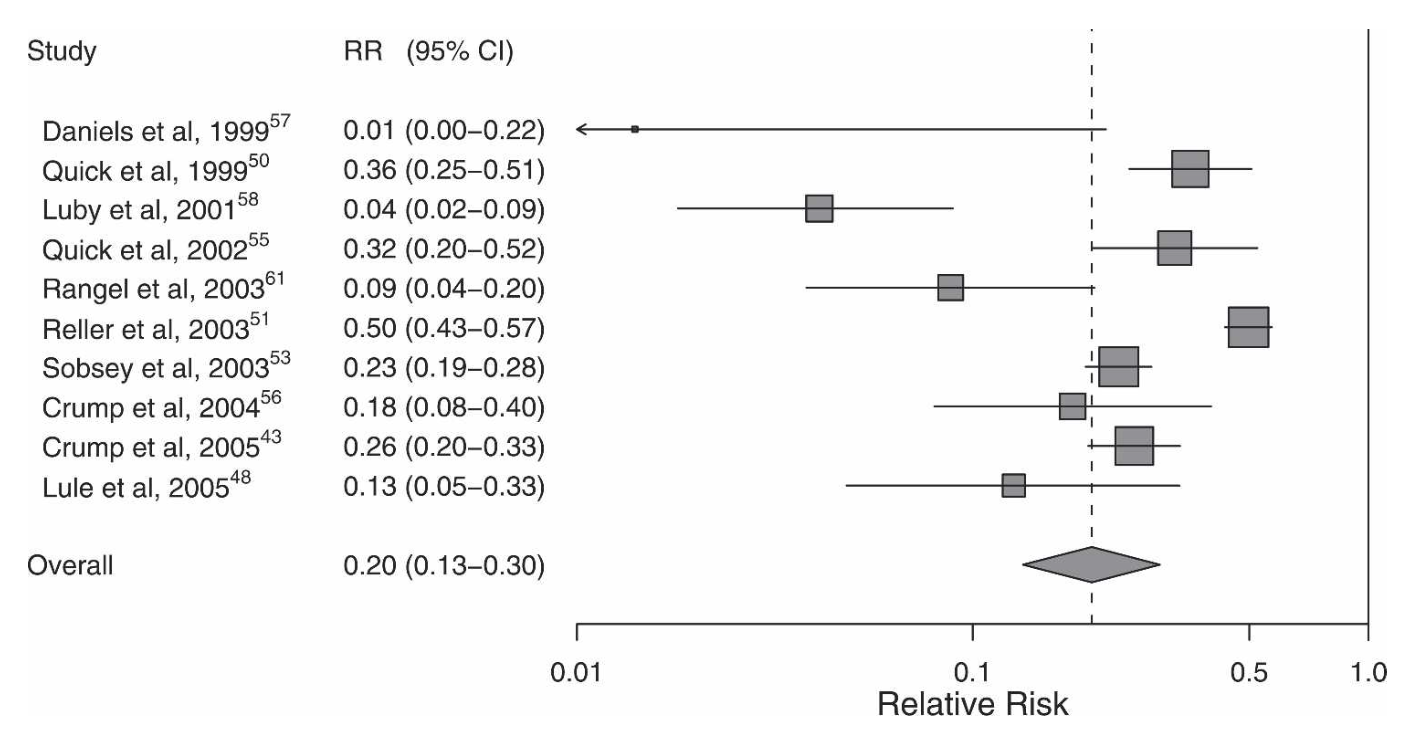
\includegraphics[width=\textwidth]{ArnoldEcoli.png}\end{subfigure}
{\footnotesize  \begin{flushleft} Notes: .\end{flushleft}}
\end{figure}

In practice, the benefits of water treatment may be attenuated outside experimental settings. Effective use of chlorine and other treatment technologies requires correct dosing and adherence to recommended procedures, which can be challenging for households. The appropriate dosage varies with baseline contamination, water turbidity, and storage conditions, and chlorine may lose potency when stored for extended periods. Even boiling does not fully ensure pathogen removal if treated water is later recontaminated during handling or storage. As a result, real-world effectiveness may fall short of laboratory efficacy estimates.

Moreover, causal evidence on water treatment largely comes from experimental settings in which households are often provided with new treatment products and, in some cases, complementary components such as education or behavior-change interventions. While these studies yield credible estimates of program impacts, their findings may not generalize to routine, non-experimental contexts where households may use treatment methods inconsistently or incorrectly, and where compliance, monitoring, and supportive activities are limited. As a result, treatment effects observed in observational settings may be smaller than those reported in controlled trials.

% E. Coli to diarrhea prevalence is clear \citep{nataro1998diarrheagenic}, there is a lack of evidence on how much of this relationship is observed in real society. 

Using the MICS data that is collected in non-experimental setting, this paper estimates the causal impact of household water treatment on E. coli contamination using Double/Debiased Machine Learning (DDML), a framework designed for settings with high-dimensional confounding. The analysis draws on MICS data from 59,633 households across 25 countries in Sub-Saharan Africa, Latin America, and Asia, incorporating objective measures of water quality. By combining flexible machine learning methods with robust causal inference techniques, the study addresses key identification challenges common in observational WASH data. A distinctive feature of the analysis is the use of direct measurements of source-water contamination, which permits estimation of treatment effects across varying baseline risk environments. 

The study finds that ABC. 
The OLS and DDML esitmates the reduction of having any E.coli of about 12 percent reduction from the mean. This estimate is 

The study contributes to the WASH and broader public health literature by advancing causal analysis in a non-experimental setting drawn from multiple countries.

First, the study applies Double/Debiased Machine Learning (DDML) to large-scale household survey data linked with scientifically measured E. coli contamination. Estimating the effects of household water treatment behaviors using observational data has long been challenged by endogeneity. In particular, omitted variables may jointly influence both treatment decisions and water quality outcomes. For example, wealthier households may be more likely to treat their water, while households facing cleaner source water may have weaker incentives to adopt treatment \citep{kamei2026water}. These factors limit the credibility of conventional OLS regression-based estimates. In addition to incorporating a high-dimensional set of observable household characteristics, a distinctive feature of the analysis is the use of direct measurements of source-water contamination as control variables. This allows comparisons among households facing similar baseline contamination risk. Controlling for source-water contamination helps mitigate concerns about unobservable confounding related to water and sanitation environments, as the contamination level of the source water captures important aspects of the underlying exposure to microbial risk. This paper contributes to the growing empirical literature employing DDML methods. [Add some papers]\footnote{In contrast to some of the earlier studies that rely on a single machine learning algorithm, the empirical strategy implements a stacked ensemble approach that combines multiple learners to improve predictive performance and robustness. This methodological choice highlights the practical advantages of modern machine learning integration for causal inference in applied microeconomic research.}

Second, another feature of the study is that the results are estimated in a non-experimental setting. Although randomized controlled trials (RCTs) and meta-analyses document substantial reductions in E. coli contamination from water treatment, experimental interventions often bundle multiple components—such as education, behavior change campaigns, or programmatic support—making it difficult to isolate specific mechanisms and assess external validity. By leveraging DDML in an observational context, this paper provides evidence on the impact of household water treatment on E. coli contamination under naturally occurring conditions.

Third, the analysis conducts a heterogeneity assessment that leverages a distinctive feature of the data: direct measurements of E. coli contamination at the source-water level drawn from multiple countries. This design allows treatment-effect heterogeneity to be examined using objective microbiological conditions rather than conventional socioeconomic proxies such as wealth, education, or rural–urban status. By exploiting variation in baseline contamination levels, the study evaluates how the effectiveness of water treatment behaviors differs across environments characterized by differing initial risk profiles with large externality.

% Recent studies suggest that passive chlorination at the point of water collection can be an effective intervention for reducing childhood diarrhoea in urban low-income settings \cite{pickering2019inline}. Automated chlorine dosers have been shown to disinfect drinking water without requiring electricity, leading to a significant reduction in diarrhoea prevalence as defined by WHO standards. Despite these technological advancements, other low-cost water treatment interventions, such as improved cookstoves and safe water devices, often fail to achieve their expected health benefits due to inconsistent adoption by low-income households \cite{ray2021towards}. This inconsistency hampers efforts to improve water quality, reduce E. Coli contamination, and decrease the prevalence of waterborne diseases such as diarrhoea. Additionally, the paper argues that shifting from household-scale interventions to utility-scale service models could ensure more reliable access to clean water and sanitation, which are vital in preventing diarrhoeal diseases. Overall, the global impact of inadequate WASH services is substantial, with an estimated 1.4 million deaths and 74 million disability-adjusted life years (DALYs) that could have been averted in 2019 through safe WASH practices \cite{Wolf2023Burden}. These findings underscore the importance of WASH interventions in addressing the global burden of diarrhoeal diseases linked to poor water quality and sanitation.

The remainder of this paper is organized as follows. Section 2 describes the data, sample construction, and empirical strategy, including the DDML framework, control variables, and the heterogeneity analysis by source-water contamination. Section 3 presents descriptive statistics on household characteristics, water treatment behavior, and microbiological water quality. Section 4 reports the main empirical results, comparing unadjusted estimates, OLS estimates, and DDML estimates, and examines heterogeneity in treatment effects across different contamination environments. Section 5 explores the relationship between water quality and child health outcomes, including diarrhea and fever. Section 6 concludes. Supporting materials, additional robustness checks, and the formal DDML framework are provided in the Appendix.

\section{Methods (Follow PLOS One writing)} 
\subsection{Sample} 
To examine the relationship between source water contamination, household water treatment decisions, and contamination in stored drinking water, we analyze the MICS household survey  \citep{mics_ecoli}. The MICS, implemented by UNICEF, are nationally representative household surveys designed to collect high-quality data on living standards. MICS are conducted primarily in low- and middle-income countries, using standardized sampling methods that ensure population-level representativeness at both national and sub-national levels. In addition to detailed information on demographics, health, and water and sanitation, MICS began incorporating objectively measured water-quality testing starting in Round 6.

We use MICS 6 surveys collected between 2017 and 2021, in which a rapid water quality testing module is available. The surveys were implemented by UNICEF in collaboration with national ministries and statistics offices. From an initial sample of 29 countries, we excluded Tuvalu, Kiribati, Tonga, and the Turks and Caicos Islands, where fewer than 1,000 households completed the water testing module, to ensure sufficient data for reliable country-level statistics.

In each MICS survey, a random subsample of households within each cluster was selected for water-quality testing (typically 5 households per cluster). Depending on the country, approximately 10–25\% of a random subsample of households were selected for the rapid water quality testing module (Table 1). Overall, 92.6\% of households completed water testing with non-missing data, and in most countries, E. coli data are available for over 80–90\% of the selected households. While non-consent was low (N= 653), water testing was occasionally not conducted due to the household’s inability to provide a water sample, partial completion, or errors in reading the test results. A comparison of household characteristics between those who completed the water testing and those who did not shows varying patterns across countries  (see online appendix in supporting document for further discussion). Thirteen additional observations were excluded from the final analytical sample because respondents reported that they did not know their household’s water treatment method.

In households selected for water testing, interviewers requested permission to collect water samples from two locations: (1) the source from which the household collects water, and (2) the stored drinking water within the household. Interviewers first asked for a sample of drinking water by requesting a glass of drinking water, and then asked to be shown the water source location in order to collect a sample directly from the water source. These water samples were analyzed for the presence of E. coli, an indicator of fecal contamination. 

The MICS survey and drinking water quality module are standardized across the countries. The protocol is developed collaboratively by the Joint Monitoring Program (JMP) and the global MICS program. An international water quality trainer, with support from national experts, led the training of field teams. National experts from regulatory agencies, research labs, or ministries of health provided technical input and oversight during fieldwork through a few field visits. Field teams obtained 100 mL samples and used portable E. coli enumeration tests consistent with UNICEF/JMP guidance; PoC taps were flushed for around 30 seconds before sampling. Water samples were analyzed for E. Coli using portable membrane filtration. Field teams filtered 100mL of water through a 0.45-µm filter, placed it on CompactDry EC growth media plates, and rehydrated it with 1mL of sample water.

Additionally, several observations were excluded due to missing information. Thirteen households were dropped because the reported water treatment method was “do not know,” and a further 5,280 households were excluded due to missing data on key covariates such as household education or wealth. \textbf{The final analytical sample covers 25 countries and includes 54,340 households.}

% The MICS survey reports \emph{E.~coli} counts censored at 100 colony-forming units (CFU) per 100 mL, so we construct two binary outcome variables: an indicator for \emph{some risk} (any contamination strictly between 0 and 100 CFU) and an indicator for \emph{very high risk} (contamination at or above the censoring threshold of 100 CFU), following international guidelines on microbiological water quality \citep{who_water_guidelines}. The treatment is a binary indicator for whether the household reports using any kind of water treatment; for tractability, we treat the different specific treatment methods as homogeneous.

\subsection{Statistical Approach}

Estimating the causal impact of household water treatment on E. coli contamination is complicated by endogeneity. Households that treat their drinking water may differ systematically from those that do not along both observable and unobservable dimensions, including socioeconomic status, education, access to infrastructure, and health knowledge. Conversely, if some households mistakenly perceive their water to be safe, their decision not to treat may bear little relationship to actual contamination levels. As a result, water-treatment behavior may be correlated with unobserved determinants of water quality, implying that conventional regression estimates may be biased, potentially leading to either overestimation or underestimation of treatment effects.

To address this concern, this paper employs Double/Debiased Machine Learning (DDML), a framework that combines the predictive power of machine learning with a rigorous causal inference framework. A naive application of machine learning to causal estimation faces three fundamental problems. First, machine learning is not immune to omitted variable bias: even when accounting for nonlinearities, the model can learn spurious relationships driven by confounders, yielding biased estimates. Second, the bias--variance tradeoff that ML models navigate---reducing predictive bias by fitting complex functions---can actually exacerbate bias in causal effect estimation, as models may overfit to correlations induced by confounders. Third, ML models are optimized to minimize prediction error for the outcome variable; they are not designed to isolate the effect of a specific treatment variable while controlling for confounders, and their objective function does not inherently distinguish between spurious correlations and true causal links.

Naively plugging in ML predictions also introduces regularization bias: any regularization penalty---whether favoring low variance (L2) or low deviance (L1)---can leak into the causal estimate, effectively underestimating the true relationship. The DDML framework addresses the second and third problems through two combined techniques, though it remains subject to the first (omitted variable bias), which we discuss in the context of the water treatment and contamination mechanisms below.

The ``double'' in DDML refers to the two nuisance-function residualization, an extension of the Frisch--Waugh--Lovell theorem, built on two ingredients:

\begin{enumerate}
\item \textbf{Neyman orthogonalization.} This provides a robust way to define scores such that small errors in specification do not contaminate the causal estimate. These errors are primarily measurement errors, but the most important application concerns deviations from the true parameters caused by regularization. Formally, Neyman orthogonality requires:
\begin{equation}
\left. \frac{\partial}{\partial \eta} \E[\phi(Z; \theta_0, \eta)] \right|_{\eta = \eta_0} = 0,
\end{equation}
meaning that regularization does not contaminate the causal estimate. This does not, however, fix omitted variable bias.

\item \textbf{Cross-fitting.} This technique minimizes overfitting by passing different training and test sets to the model. We implement $K$-fold cross-fitting, which divides the full dataset into $K$ disjoint subsamples. For each fold, the model trains on $K-1$ subsamples and predicts on the held-out subsample to obtain score values. The process is repeated iteratively, and $\hat{\theta}$ is estimated by aggregating all score results across folds.
\end{enumerate}

A commonly used score is the AIPW (Augmented Inverse Probability Weighting) score function, which is doubly robust---equivalent in spirit to Neyman orthogonality---in the sense that it remains consistent if either the outcome model or the propensity score model is correctly specified.

We employ the Interactive Regression Model (IRM) to capture the complex reality of heterogeneous treatment effects. The IRM allows the treatment effect to vary with covariates:

\begin{equation}
Y = g_0(D, X) + \varepsilon,
\end{equation}
where the treatment effect is no longer constant but a function of the covariates $X$, known as the Conditional Average Treatment Effect (CATE), which may be either linear or nonlinear.


\subsection{Causal Chain}

We identify the following causal chain:
\begin{equation}
M_{\text{source}} \to T \to M_{\text{drinking}} \to Y,
\end{equation}
where $M_{\text{source}}$ is the baseline water quality measured as CFU \textit{E. coli} count, discretized as: 0 = No risk (0 CFU), 1 = Some risk ($1 \leq \text{CFU} < 100$), and 2 = Very high risk (CFU $\geq$ 100). This discretization is motivated by the fact that the original water quality variables are right-censored at 101 CFU.

$T$ denotes the treatment variable. We evaluate two treatment specifications: (1) \textit{Any treatment}: a binary indicator (0 = no treatment, 1 = any treatment), and (2) \textit{Multitreatment}: categorical treatment by type---boil, chlorine, filter, or other---each compared to the control (no treatment).

An important identification insight concerns the role of $M_{\text{source}}$. If we ignore the path $M_{\text{source}} \to T$, we end up comparing ``clean-source'' households who do not treat with ``dirty-source'' households who do treat. Because those who treat water are systematically starting from a worse baseline, a simple comparison would underestimate the effectiveness of treatment, as $M_{\text{source}}$ acts as a confounder. Conversely, conditioning on $M_{\text{drinking}}$ in the base model would block the biological pathway (it acts as a mediator), which would lead to observing no treatment effect. Our empirical strategy therefore controls for $M_{\text{source}}$ but does not condition on $M_{\text{drinking}}$.







\subsection{Characteristics associated with household water treatment (JA To update: Not it is Logit model)}
To characterize the factors associated with household water treatment, this study employs a LASSO-regularized linear probability model. Water treatment decisions are likely influenced by a large set of household, environmental, and infrastructural characteristics, many of which are highly correlated. Including all such covariates in a conventional regression risks overfitting and unstable estimates.

LASSO provides a data-driven approach to variable selection by shrinking the coefficients of less informative covariates toward zero, retaining only those predictors most strongly associated with water treatment behavior. We estimate a linear probability model of water treatment on a high-dimensional set of pre-treatment household and community characteristics, using LASSO regularization to identify the most relevant correlates. The linear specification is chosen for computational stability and compatibility with the subsequent causal machine learning framework.

The purpose of this exercise is not causal inference, but descriptive: to summarize which observable characteristics are most predictive of household water treatment and to inform the selection of controls used in the causal analysis. 

\subsection{Causal impact of water treatment on E. coli reduction in household water}

The double/debiased machine-learning framework allows flexible adjustment for confounding factors by using machine-learning methods to estimate high-dimensional nuisance components. This approach accommodates nonlinearities and interactions among covariates without imposing restrictive functional-form assumptions (see Appendix \ref{DDMLTheo} for the formal explanation).

The key identifying assumption is conditional independence: conditional on the observed covariates $X_i$, the household's water-treatment decision is assumed to be independent of unobserved determinants of drinking-water contamination. After controlling for a rich set of household and environmental characteristics, treatment status is therefore interpreted as being as good as randomly assigned with respect to latent contamination risk.

Under the Neyman-orthogonality and rate conditions discussed above, DDML corrects for regularization and overfitting biases in high-dimensional first-stage models, yielding debiased estimates of the treatment effect. We implement DDML using the \texttt{DoubleML} package for R \citep{doubleml2022}, which implements the framework of \citet{chernozhukov2018double}. The stacked ensemble is constructed using \texttt{mlr3pipelines} \citep{mlr3pipelines}, which allows flexible composition of base learners and meta-learners.

Concretely, for each outcome (some risk and very high risk), we consider several first-stage learners: a linear model (OLS for the outcome regression, logistic regression for the propensity score), penalized linear models (lasso, ridge, and elastic net, each tuned via cross-validation of the regularization parameter using \texttt{cv\_glmnet}), and nonlinear tree-based methods (random forest via \texttt{ranger} with 500 trees, and gradient boosting via \texttt{xgboost} with 300 rounds, maximum depth of 4, learning rate of 0.1, subsample ratio of 0.8, and column subsample ratio of 0.8). All learners are specified for both the outcome model $E[Y \mid X, D]$ and the treatment propensity model $E[D \mid X]$, with classification variants (logistic variants for linear models, probabilistic prediction for tree-based methods) used for the binary propensity score. In addition, we construct a \textit{stacked} ensemble learner: each base learner generates cross-validated out-of-fold predictions, which are combined via feature union and passed to a ridge regression meta-learner (\texttt{cv\_glmnet} with $\alpha = 0$) that selects optimal stacking weights by minimizing out-of-sample loss. Final stacking weights are reported as the normalized absolute coefficients of the ridge meta-learner.

An important feature of our specification concerns the inclusion of source-water E. coli controls. For diarrhea outcomes, source-water contamination dummies are included as confounders, since they plausibly affect both treatment adoption and child health. For E. coli contamination outcomes, however, source-water contamination is \textit{not} included: it lies on the causal pathway from treatment to the outcome (i.e., it is a mediator rather than a confounder), and conditioning on it would block the effect of interest.

OLS estimates are excluded from specific-treatment panels due to quasi-complete separation: country fixed effects perfectly predict zero treatment in several countries (e.g., Benin and Central African Republic have a 0\% boil rate), causing infinite MLE in the logistic propensity model and rank-deficient fits in the outcome model. Regularized learners (lasso, ridge, elastic net) are unaffected, as penalties prevent coefficient divergence. The stacked ensemble for specific treatments uses only five base learners (lasso, ridge, elastic net, random forest, XGBoost) to avoid OLS contamination. Cross-fitting is implemented with $K = 5$ folds and 2 repetitions.



\subsection{Control Variables}

This study reports three sets of estimates: (1) OLS estimates with controls, and (2) Double/Debiased Machine Learning (DDML) estimates using the same set of control variables as in the OLS specification.

The control vector includes the following household and environmental characteristics. Household wealth is captured by a set of five wealth-index quintile dummies. The education of the household head is represented by five dummies corresponding to none, primary, lower secondary, upper secondary, and college education, plus a category for missing values. Urban residence is indicated by a binary variable. Water source type is captured by 15 detailed dummies corresponding to the MICS classification: piped water into the dwelling, piped water to yard/plot, piped water to neighbor, public tap/standpipe, tube well/borehole, protected well, unprotected well, protected spring, unprotected spring, rainwater, tanker-truck, cart with small tank, surface water, bottled water, and other. Sanitation is captured by a binary indicator for improved latrine facilities. The number of children in the household (0, 1, or 2) is included to account for differences in exposure, water use, and hygiene practices. Country fixed effects (25 dummies) are included to account for cross-country heterogeneity.

The same set of control variables is included in both the outcome model and the propensity score model of the DDML framework, with one important exception: for diarrhea outcomes, source-water E.\,coli risk dummies (no risk, moderate, very high) are included as confounders, since source contamination plausibly affects both treatment adoption and child health. For E.\,coli contamination outcomes, however, source-water contamination is \textit{not} included as a control, as it lies on the causal pathway from treatment to the outcome (i.e., it is a mediator rather than a confounder), and conditioning on it would block the effect of interest.


\subsection{Subsample analysis and heterogeneity by source-water contamination}

A central advantage of the MICS data is the availability of direct measures of \emph{E.~coli} contamination at the household’s water source. This allows us to examine heterogeneity in the effectiveness of household water treatment by baseline microbial risk, a dimension that is conceptually important for identification and interpretation. Treatment technologies are expected to have limited impact when source water is uncontaminated, while their potential benefits should be larger when households are exposed to higher contamination levels.

We stratify households according to baseline source-water contamination (rather than point-of-use samples). Low-risk sources are defined as 0 CFU of \emph{E.~coli}, moderate-risk sources as 1–100 CFU, and high-risk sources as more than 100 CFU per 100 mL. For households drawing from low-risk sources, we expect little or no treatment effect, as there is essentially no contamination to remove. In contrast, for households exposed to moderate or high contamination, larger reductions in \emph{E.~coli} are expected unless treatment practices are inefficient (e.g.\ incorrect or inconsistent application) or environmental contamination is sufficiently severe to offset treatment effectiveness.

In the full sample of 54,340 households, 23,079 households rely on low-risk sources, 19,648 households are exposed to moderate contamination, and 11,613 households draw from highly contaminated sources. The corresponding DDML estimates for each subsample are reported in Tables X and Y, with stacking weights shown in Table~Z.

\section{Descriptive Statistics}\label{Descriptive}\setcounter{figure}{0}\setcounter{table}{0}
Table \ref{Desc1} presents household characteristics and water treatment behavior based on the contamination level of the source water. The final sample size is \ToTSample{} households from 25 countries, with 25,518 (43 percent) in the low-risk category, 21,844 (37 percent) in the moderate-risk category, and 12,271 (21 percent) in the very high-risk category at the water source. 

%-------------------------------------------------------------%
{\renewcommand\normalsize{}\normalsize\singlespacing  
\begin{table}[htbp]\centering
\def\sym#1{\ifmmode^{#1}\else\(^{#1}\)\fi}
\caption{Household Characteristics by Water Source Contamination Level, extended (share) \label{Desc1}}
\begin{tabular}{l*{6}{c}}
\hline\hline
                    &\multicolumn{1}{c}{Low risk}&\multicolumn{1}{c}{Moderate risk}&\multicolumn{1}{c}{High risk}&\multicolumn{1}{c}{model6}&\multicolumn{1}{c}{model7}&\multicolumn{1}{c}{model8}\\
                    &           _&           _&           _&           _&           _&           _\\
\hline
Any treatment (Water tested)&        0.23&        0.20&        0.22&        0&        1&        0\\
~~~ Nothing      &        0.77&        0.80&        0.78&        0&        1&        0\\
~~~ Boil         &        0.12&        0.08&        0.08&        0&        1&        0\\
~~~ Chlorine/Aquatabs/PUR&        0.01&        0.03&        0.03&        0&        1&        0\\
~~~ Strain/Settle&        0.03&        0.06&        0.08&        0&        1&        0\\
~~~ Other        &        0.05&        0.04&        0.03&        0&        1&        0\\
\textbf{Household socioeconomic status} \\\hline Poorest quintile             &        0.13&        0.23&        0.31&        0&        1&        0\\
Poor                &        0.16&        0.21&        0.24&        0&        1&        0\\
Middle quintile              &        0.20&        0.20&        0.20&        0&        1&        0\\
Rich                &        0.23&        0.20&        0.15&        0&        1&        0\\
Richest quintile             &        0.28&        0.17&        0.10&        0&        1&        0\\
\textbf{HH Education} \\\hline No education        &        0.15&        0.25&        0.35&        0&        1&        0\\
Primary             &        0.25&        0.32&        0.34&        0&        1&        0\\
Second quintileary or higher &        0.53&        0.41&        0.30&        0&        1&        0\\
Missing             &        0.07&        0.02&        0.01&        0&        1&        0\\
\textbf{Primary water source} \\\hline Piped connection         &        0.41&        0.30&        0.17&        0&        1&        0\\
Tube/Well/Borehole  &        0.27&        0.28&        0.12&        0&        1&        0\\
Protected well or spring/spring&        0.03&        0.09&        0.14&        0&        1&        0\\
Unprotected well or spring/spring&        0.02&        0.11&        0.30&        0&        1&        0\\
Surface/Rain water  &        0.02&        0.07&        0.18&        0&        1&        0\\
Packaged/Bottled water&        0.21&        0.14&        0.07&        0&        1&        0\\
Others              &        0.03&        0.01&        0.01&        0&        1&        0\\
\textbf{Household Demographic} \\\hline Have U5 children    &        0.35&        0.42&        0.51&        0&        1&        0\\
Girls_less_than15   &        0.02&        0.04&        0.06&        0&        1&        0\\
Boys_15or_less      &        0.01&        0.02&        0.02&        0&        1&        0\\
Urban               &        0.54&        0.35&        0.24&        0&        1&        0\\
Flush toilet        &        0.54&        0.41&        0.24&        0&        1&        0\\
Pit latrine         &        0.38&        0.40&        0.36&        0&        1&        0\\
Open defecation     &        0.06&        0.16&        0.36&        0&        1&        0\\
Missing / not observed&        0.01&        0.02&        0.04&        0&        1&        0\\
\textbf{Water test results} \\\hline Source sample (CFU/100mL)&        0&       21.10&      101&        0&      101&        0\\
Household water test (100ml)&       17.80&       44.27&       86.11&        0&      101&        0\\
\hline
N                   &      25,511&      21,841&      12,268&      59,620&      59,620&      59,620\\
\hline\hline
\multicolumn{7}{p{0.96\linewidth}}{\footnotesize Notes: The table presents extended household characteristics across 25 countries. The number of CFUs per 100mL of E. coli is capped at 101 if the number is higher than 100. The mean of the blank water test is 0.67 CFUs per 100mL.}\\
\end{tabular}
\end{table}

}
%-------------------------------------------------------------% 


\clearpage
\section{Empirical Results}\label{Empirical}
The main DDML estimates for the PLM parameter are reported in Tables~\ref{SR_plm} and~\ref{VH_plm}, which show, for each nuisance specification and control set, the estimated effect of household water treatment on the probability of being in the \emph{some risk} and \emph{very high risk} categories, respectively. Table~\ref{w_plm} reports the corresponding stacking weights assigned to each base learner in the preferred DDML specification, indicating which algorithms contribute most to the final, debiased estimates.

This section presents the ordinary least squares (OLS) estimates as a benchmark, followed by results from the Double/Debiased Machine Learning (DDML) framework using both the partially linear and interactive specifications.

\subsection{Characteiristics assocaited with Water Treatment}\label{LASSO}

JA: Please add Logit results

\subsection{OLS and DDML}\label{OLS}

Tables \ref{tab:Est_EColi_OLS_SomeRiskHome_full} and \ref{tab:Est_EColi_OLS_VeryHighRiskHome_full} present ordinary least squares (OLS) estimates of the association between household water treatment and \textit{E. coli} contamination in household drinking water, using the same set of control variables and stratifying households by the level of \textit{E. coli} risk at the water source.

Table \ref{tab:Est_EColi_OLS_SomeRiskHome_full} focuses on the probability that any \textit{E. coli} is detected in household drinking water. Among households with no detectable \textit{E. coli} at the source, 23,595 households are included in the sample, yet approximately 50 percent (see the mean of the dependent variable) exhibit some \textit{E. coli} contamination at the point of use. Water treatment is associated with a statistically significant reduction of 7.3 percentage points in the probability of \textit{E. coli} detection. The estimated reduction is larger among households whose source water contains moderate contamination levels (1–100 CFU). In contrast, the estimated effects are smaller for households facing high-risk source contamination, potentially reflecting recontamination during storage or inappropriate treatment practices, as chlorine is less effective under high organic load or incorrect dosing.


%-------------------------------------------------------------%
{\renewcommand\normalsize{\small}\normalsize\singlespacing  
\input{Table/Est_EColi_OLS_SomeRiskHome_full.tex}
}  
%-------------------------------------------------------------% 

Table \ref{tab:Est_EColi_OLS_VeryHighRiskHome_full} examines the probability that household drinking water contains very high \textit{E. coli} contamination levels (greater than 100 CFU). Overall, water treatment does not significantly reduce the probability of very high contamination in households whose source water is classified as low risk. This is partly mechanical: only about 14 percent of these households exhibit very high contamination at the point of use, limiting scope for detectable treatment effects. However, the estimated effect of water treatment becomes larger in magnitude as source contamination risk increases, suggesting that treatment effectiveness is more pronounced when households are exposed to higher baseline microbial risk at the source.

%-------------------------------------------------------------%
{\renewcommand\normalsize{\small}\normalsize\singlespacing  
\input{Table/Est_EColi_OLS_VeryHighRiskHome_full.tex}
}  
%-------------------------------------------------------------% 

\begin{itemize}
	\item Some risk: Smaller than OLS
	\item High risk: Larger than OLS
\end{itemize}


\begin{figure}[htbp]\centering
\caption{Coefplot}\label{Result1}
%\begin{subfigure}[b]{0.9\textwidth}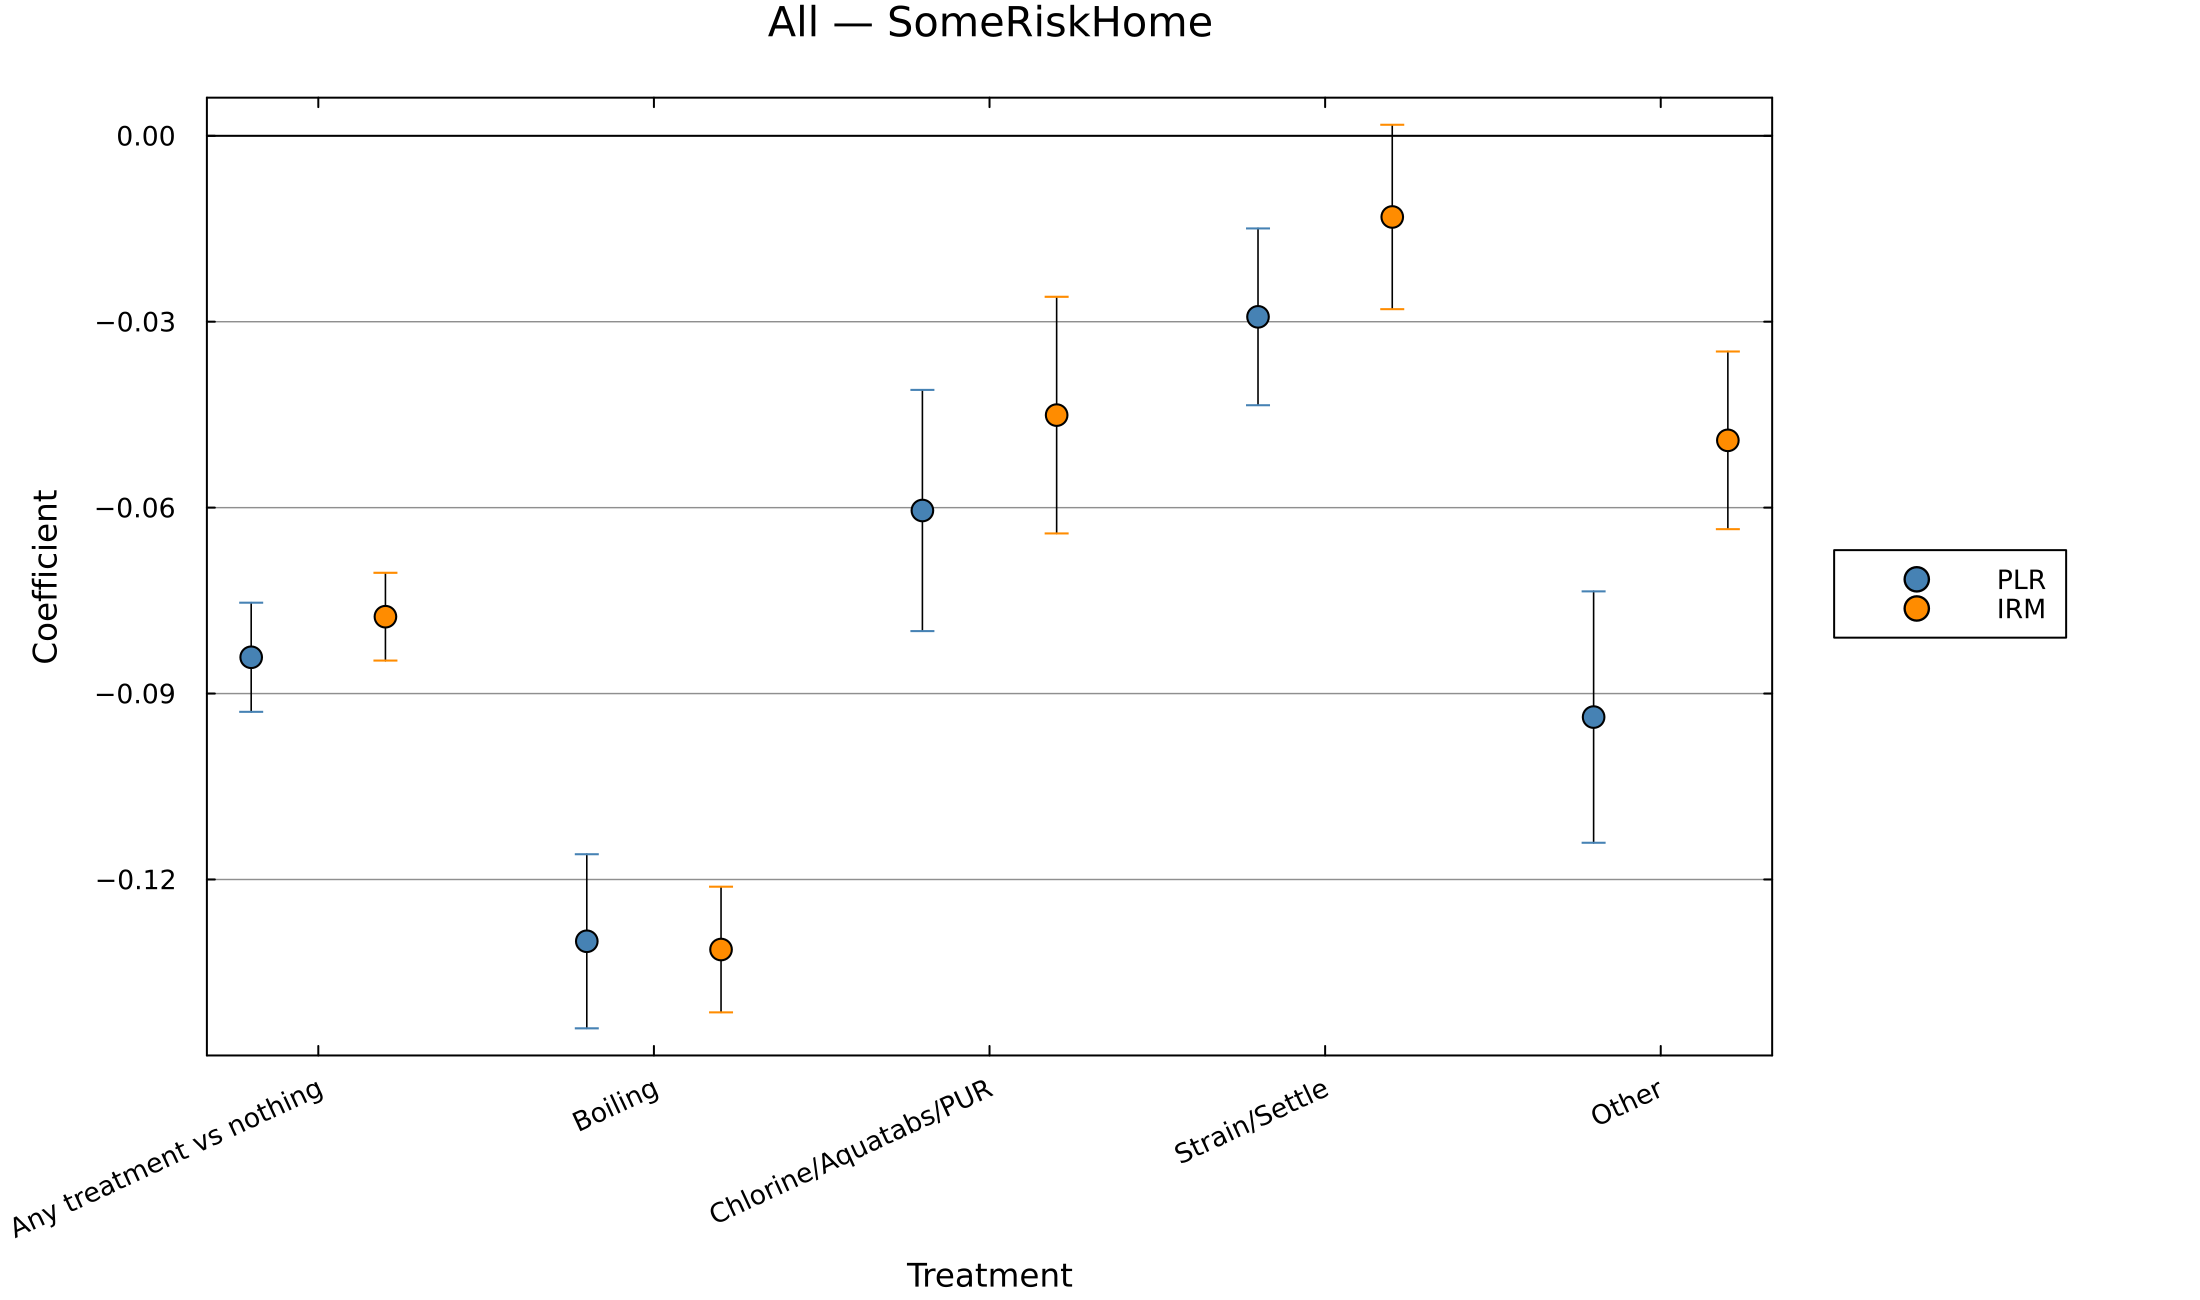
\includegraphics[width=\textwidth]{coefplot_Treatments_All_SomeRiskHome_PLR_IRM.png}\end{subfigure}
%\begin{subfigure}[b]{0.9\textwidth}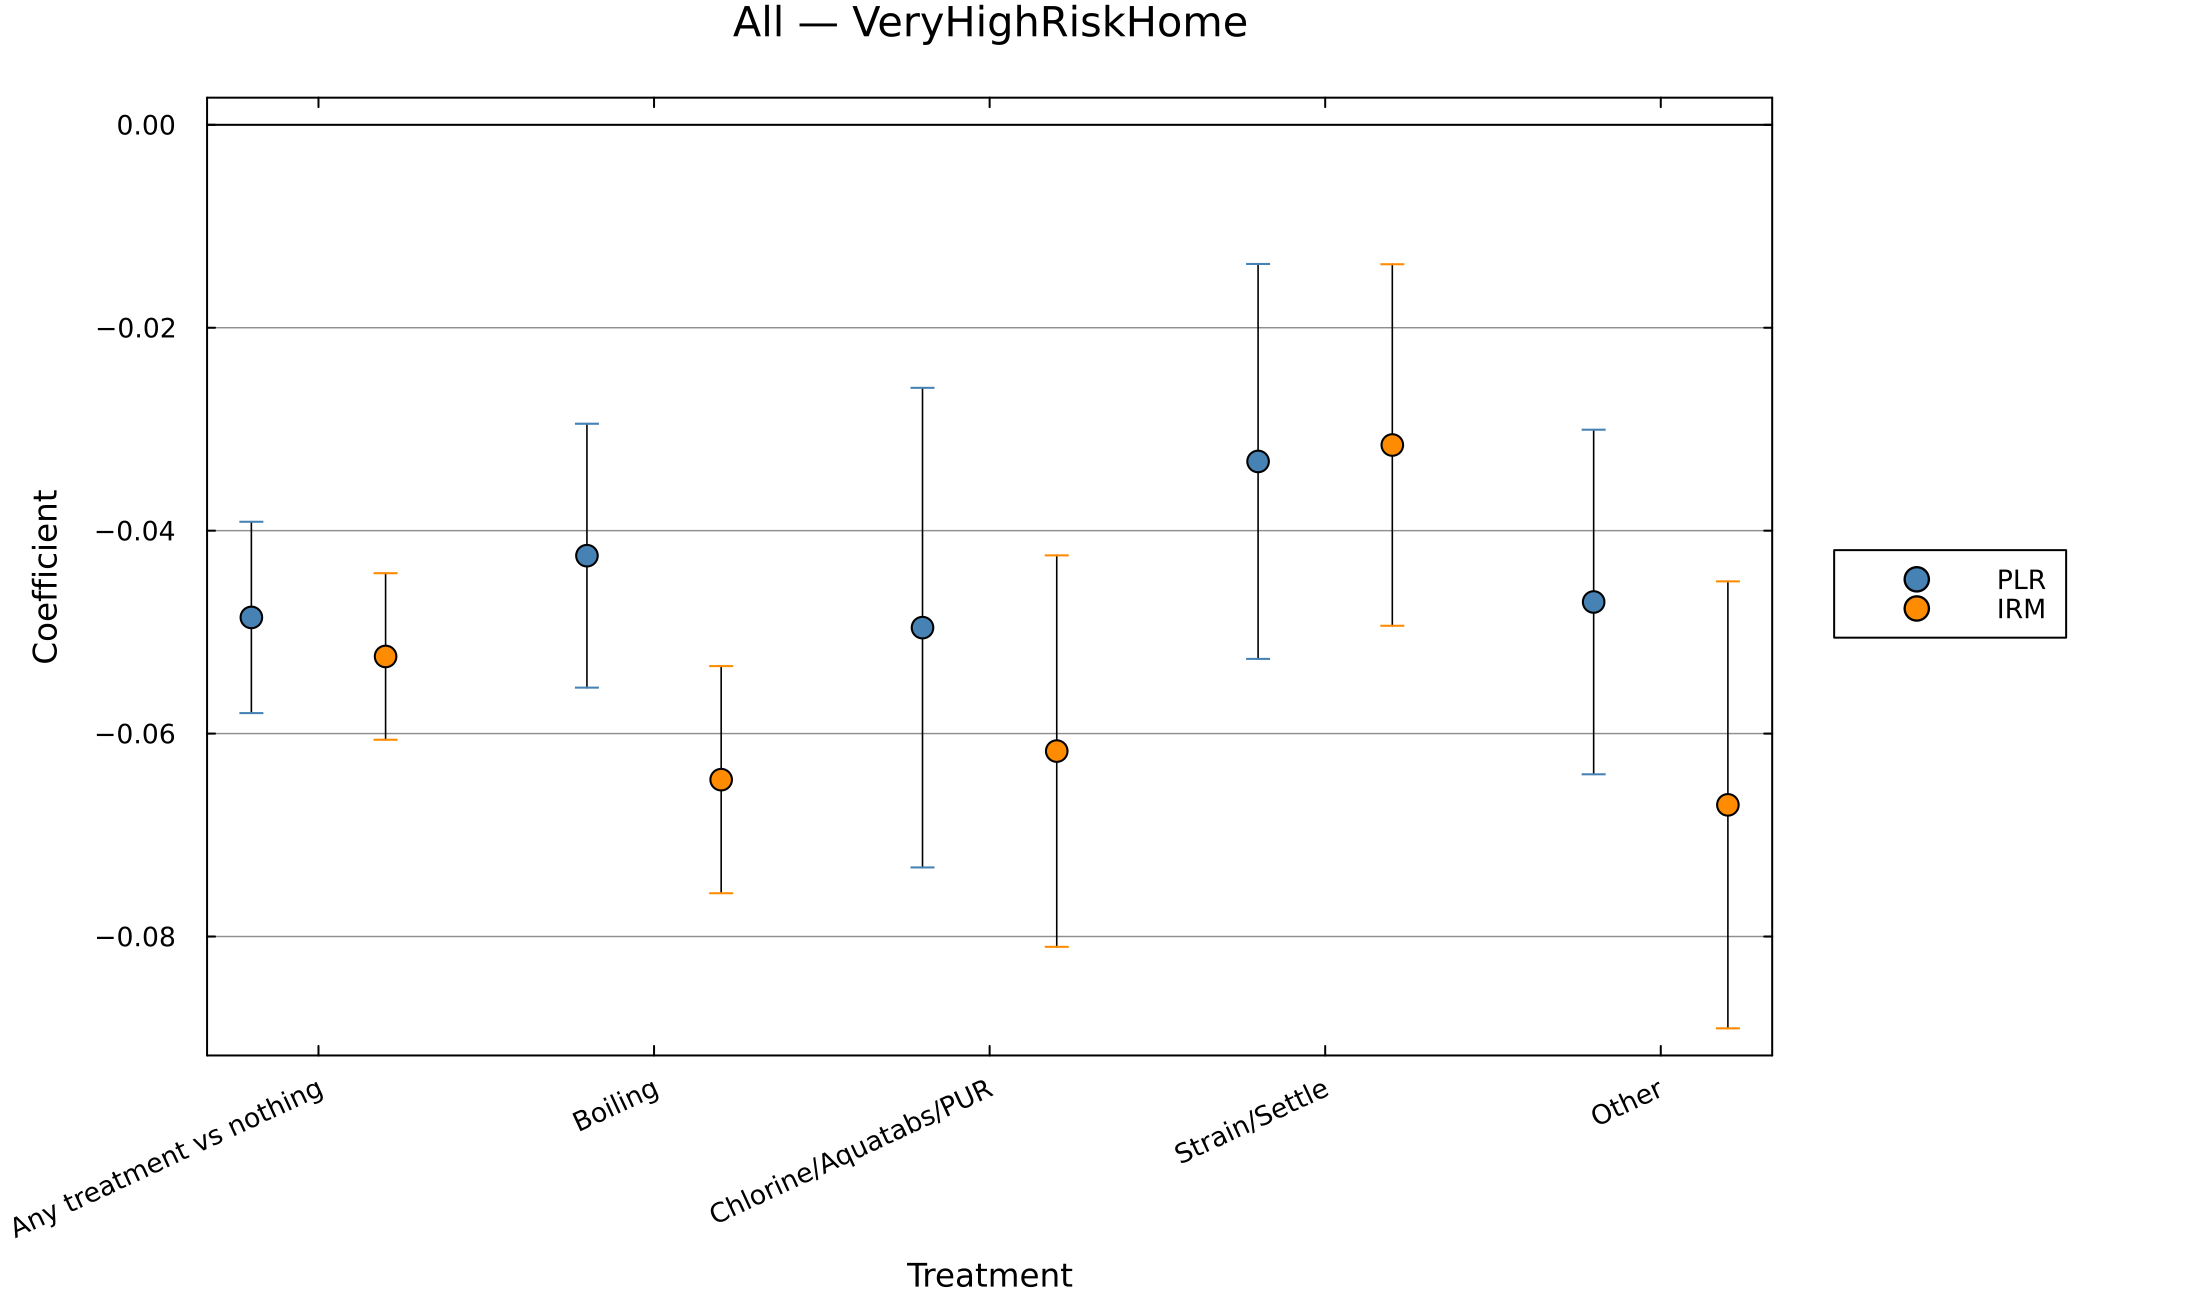
\includegraphics[width=\textwidth]{coefplot_Treatments_All_VeryHighRiskHome_PLR_IRM.png}\end{subfigure}
{\footnotesize  \begin{flushleft} Notes: .\end{flushleft}}
\end{figure}


\begin{figure}[htbp]\centering
\caption{Coefplot}\label{Result1}
%\begin{subfigure}[b]{0.7\textwidth}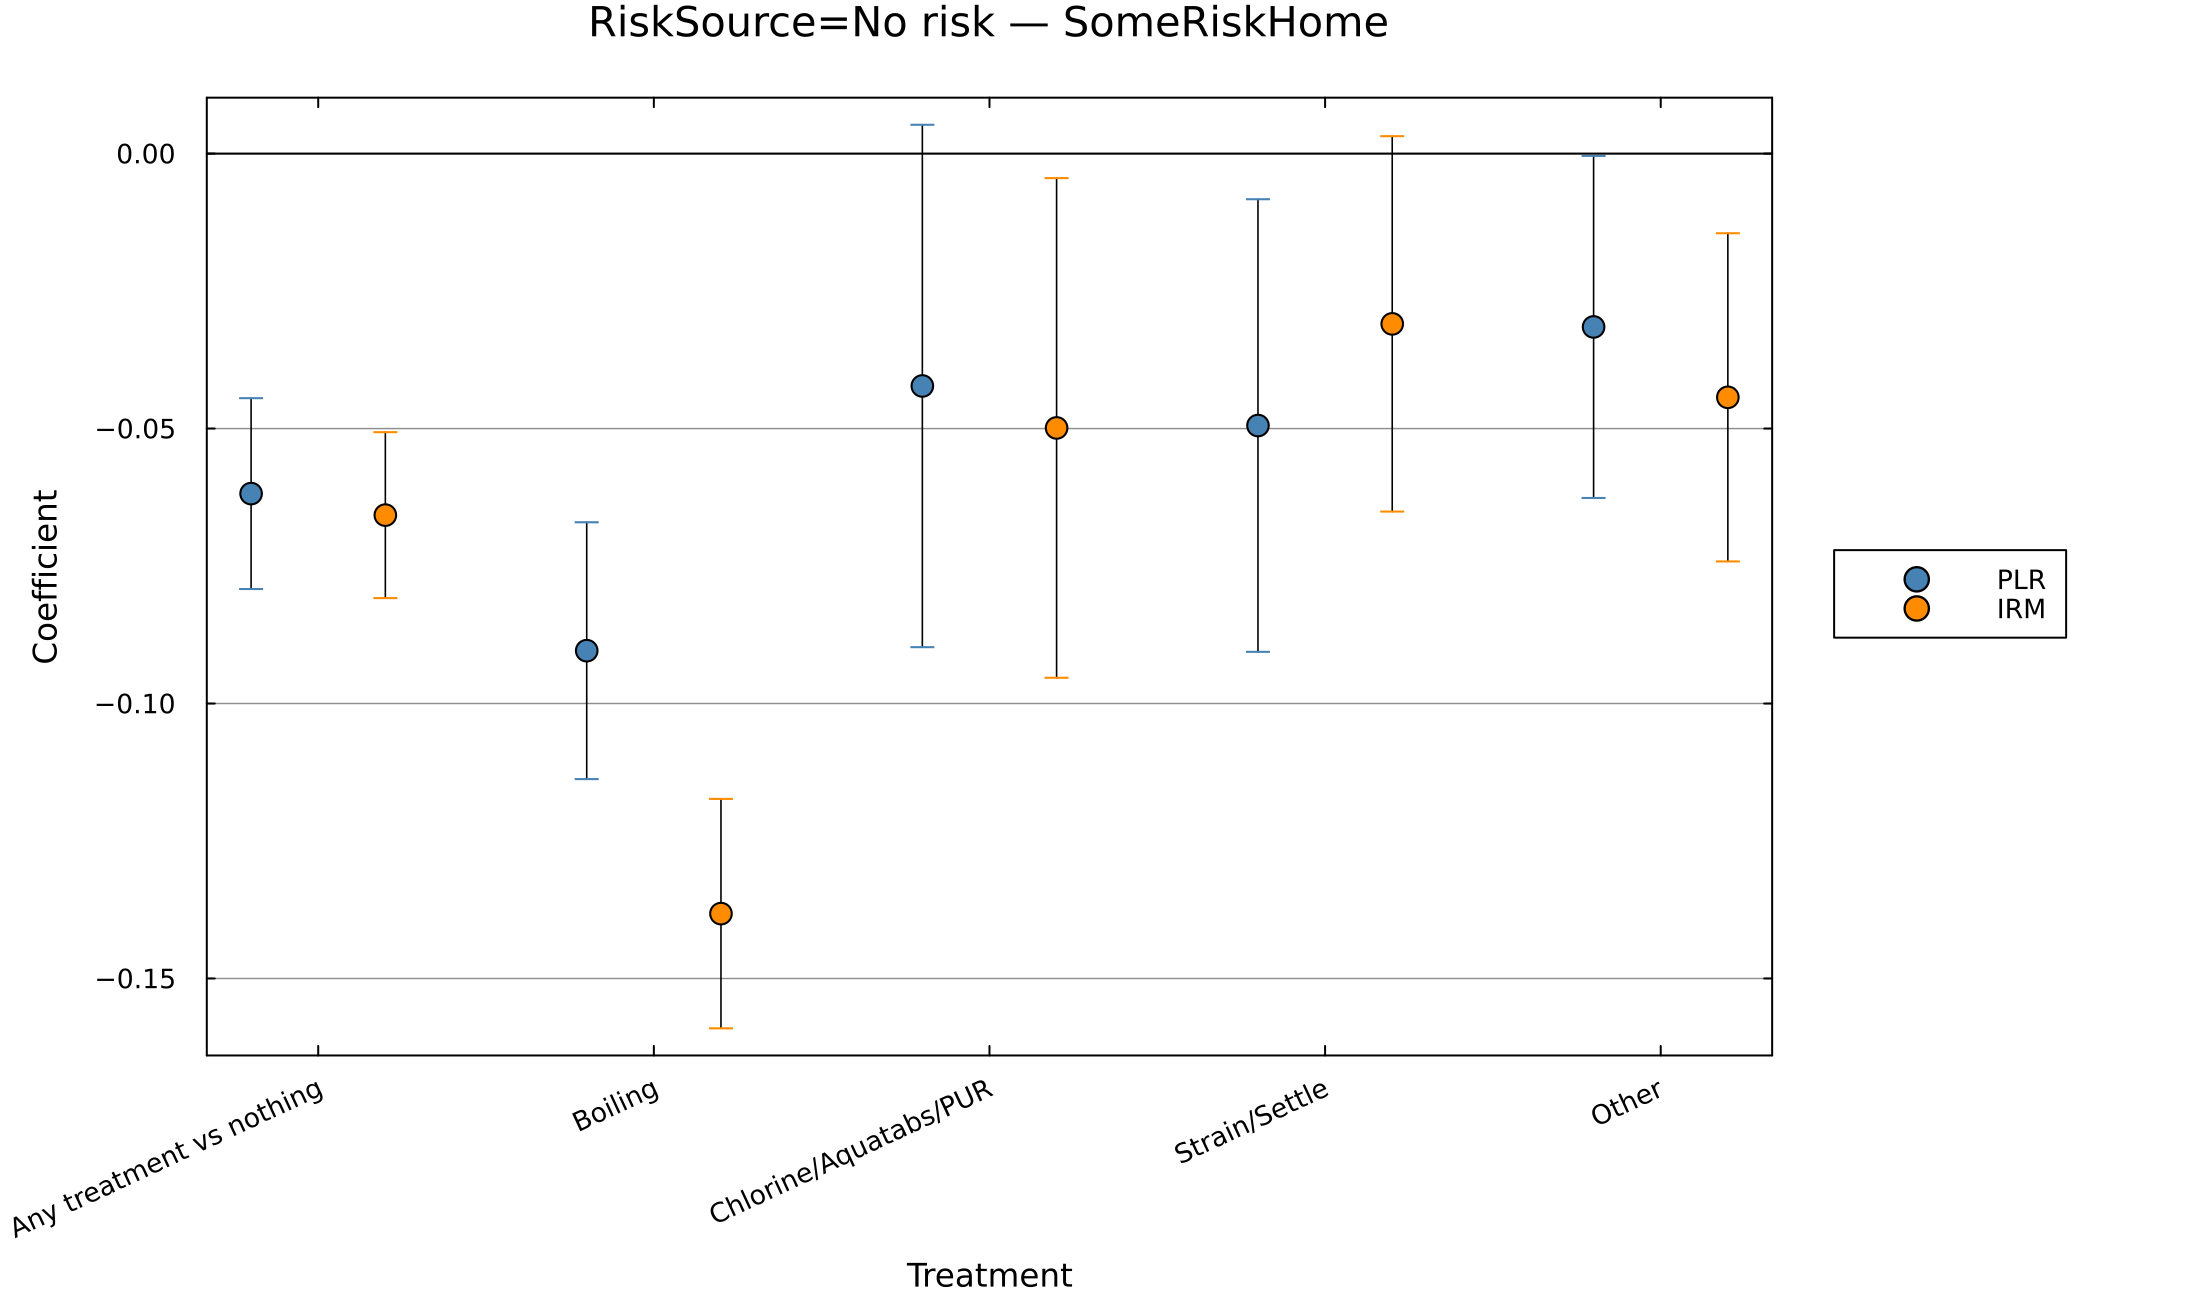
\includegraphics[width=\textwidth]{coefplot_Treatments_RiskSourceNo_risk_SomeRiskHome_PLR_IRM.png}\end{subfigure}
%\begin{subfigure}[b]{0.7\textwidth}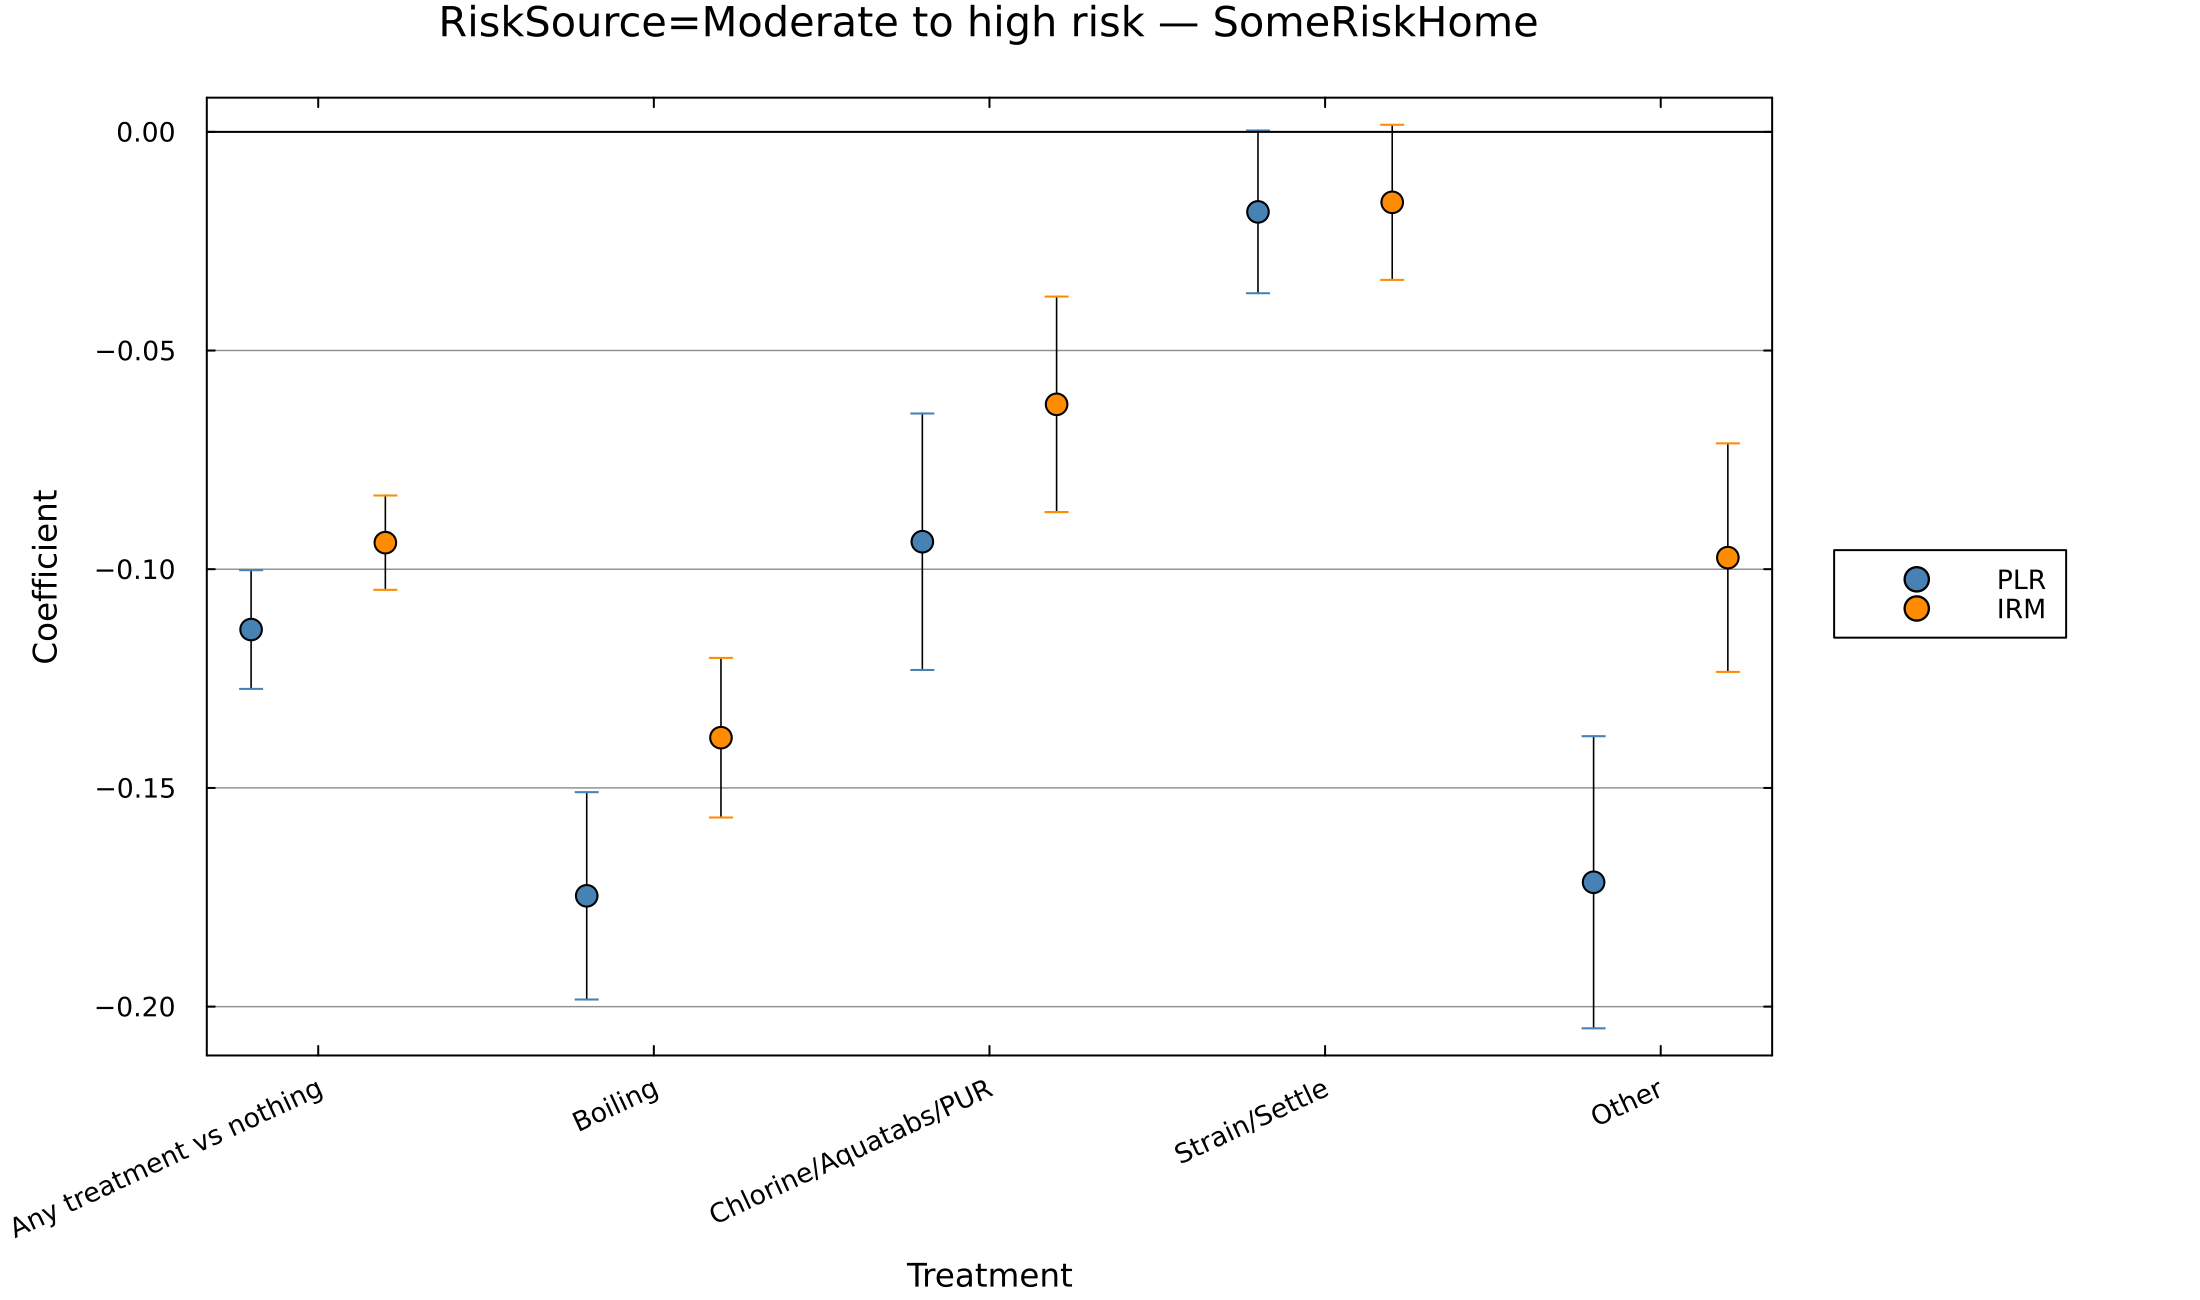
\includegraphics[width=\textwidth]{coefplot_Treatments_RiskSourceModerate_to_high_risk_SomeRiskHome_PLR_IRM.png}\end{subfigure}
%\begin{subfigure}[b]{0.7\textwidth}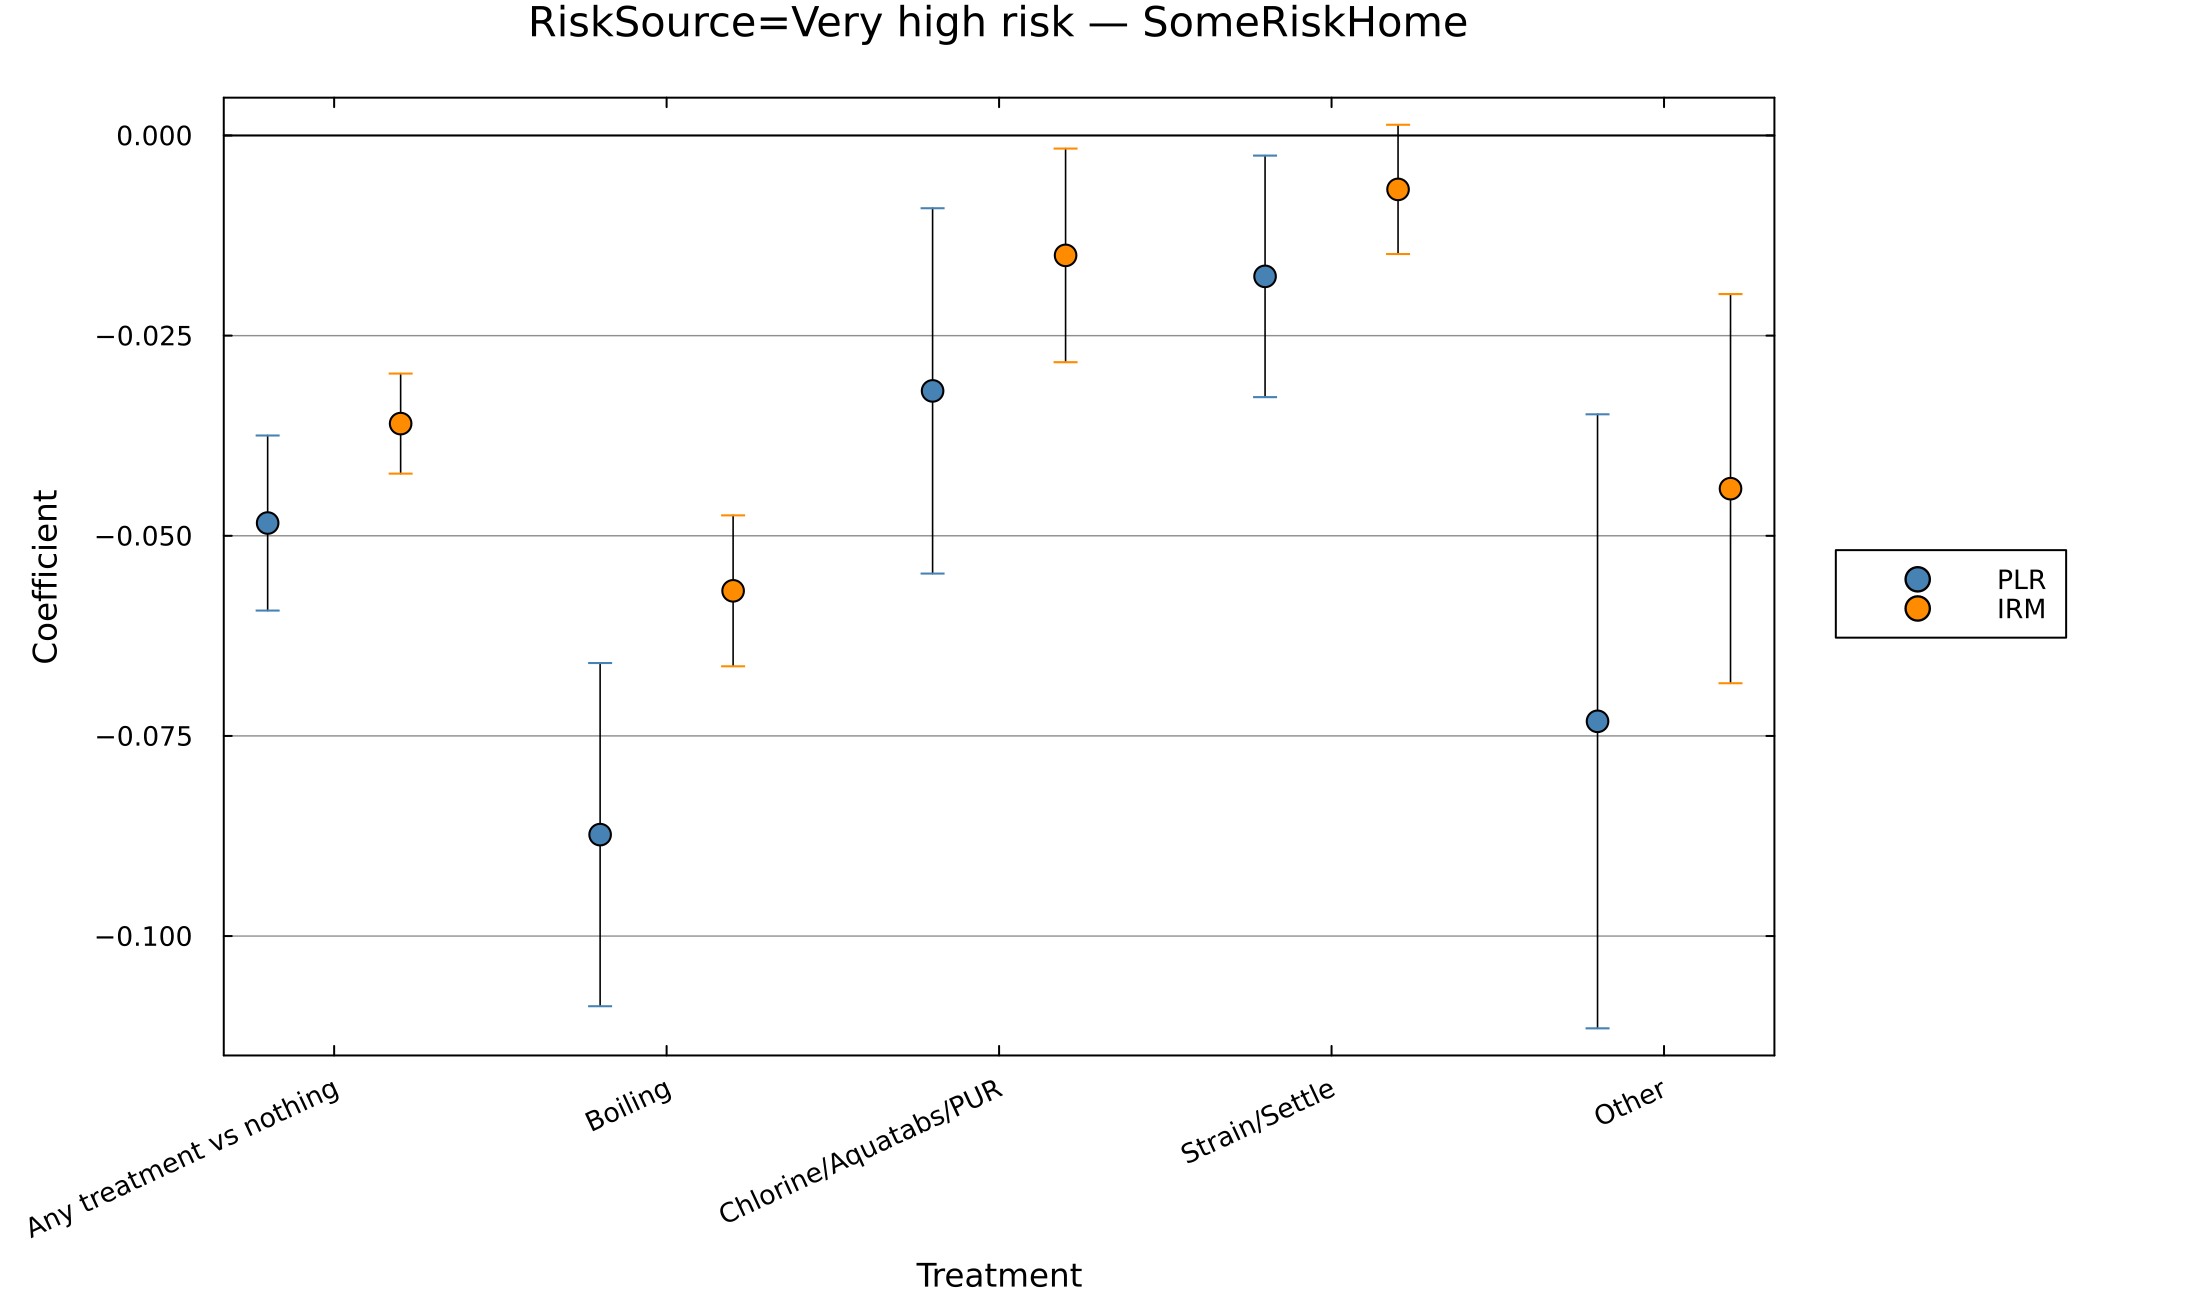
\includegraphics[width=\textwidth]{coefplot_Treatments_RiskSourceVery_high_risk_SomeRiskHome_PLR_IRM.png}\end{subfigure}
{\footnotesize  \begin{flushleft} Notes: .\end{flushleft}}
\end{figure}

\begin{figure}[htbp]\centering
\caption{Coefplot}\label{Result1}
%\begin{subfigure}[b]{0.7\textwidth}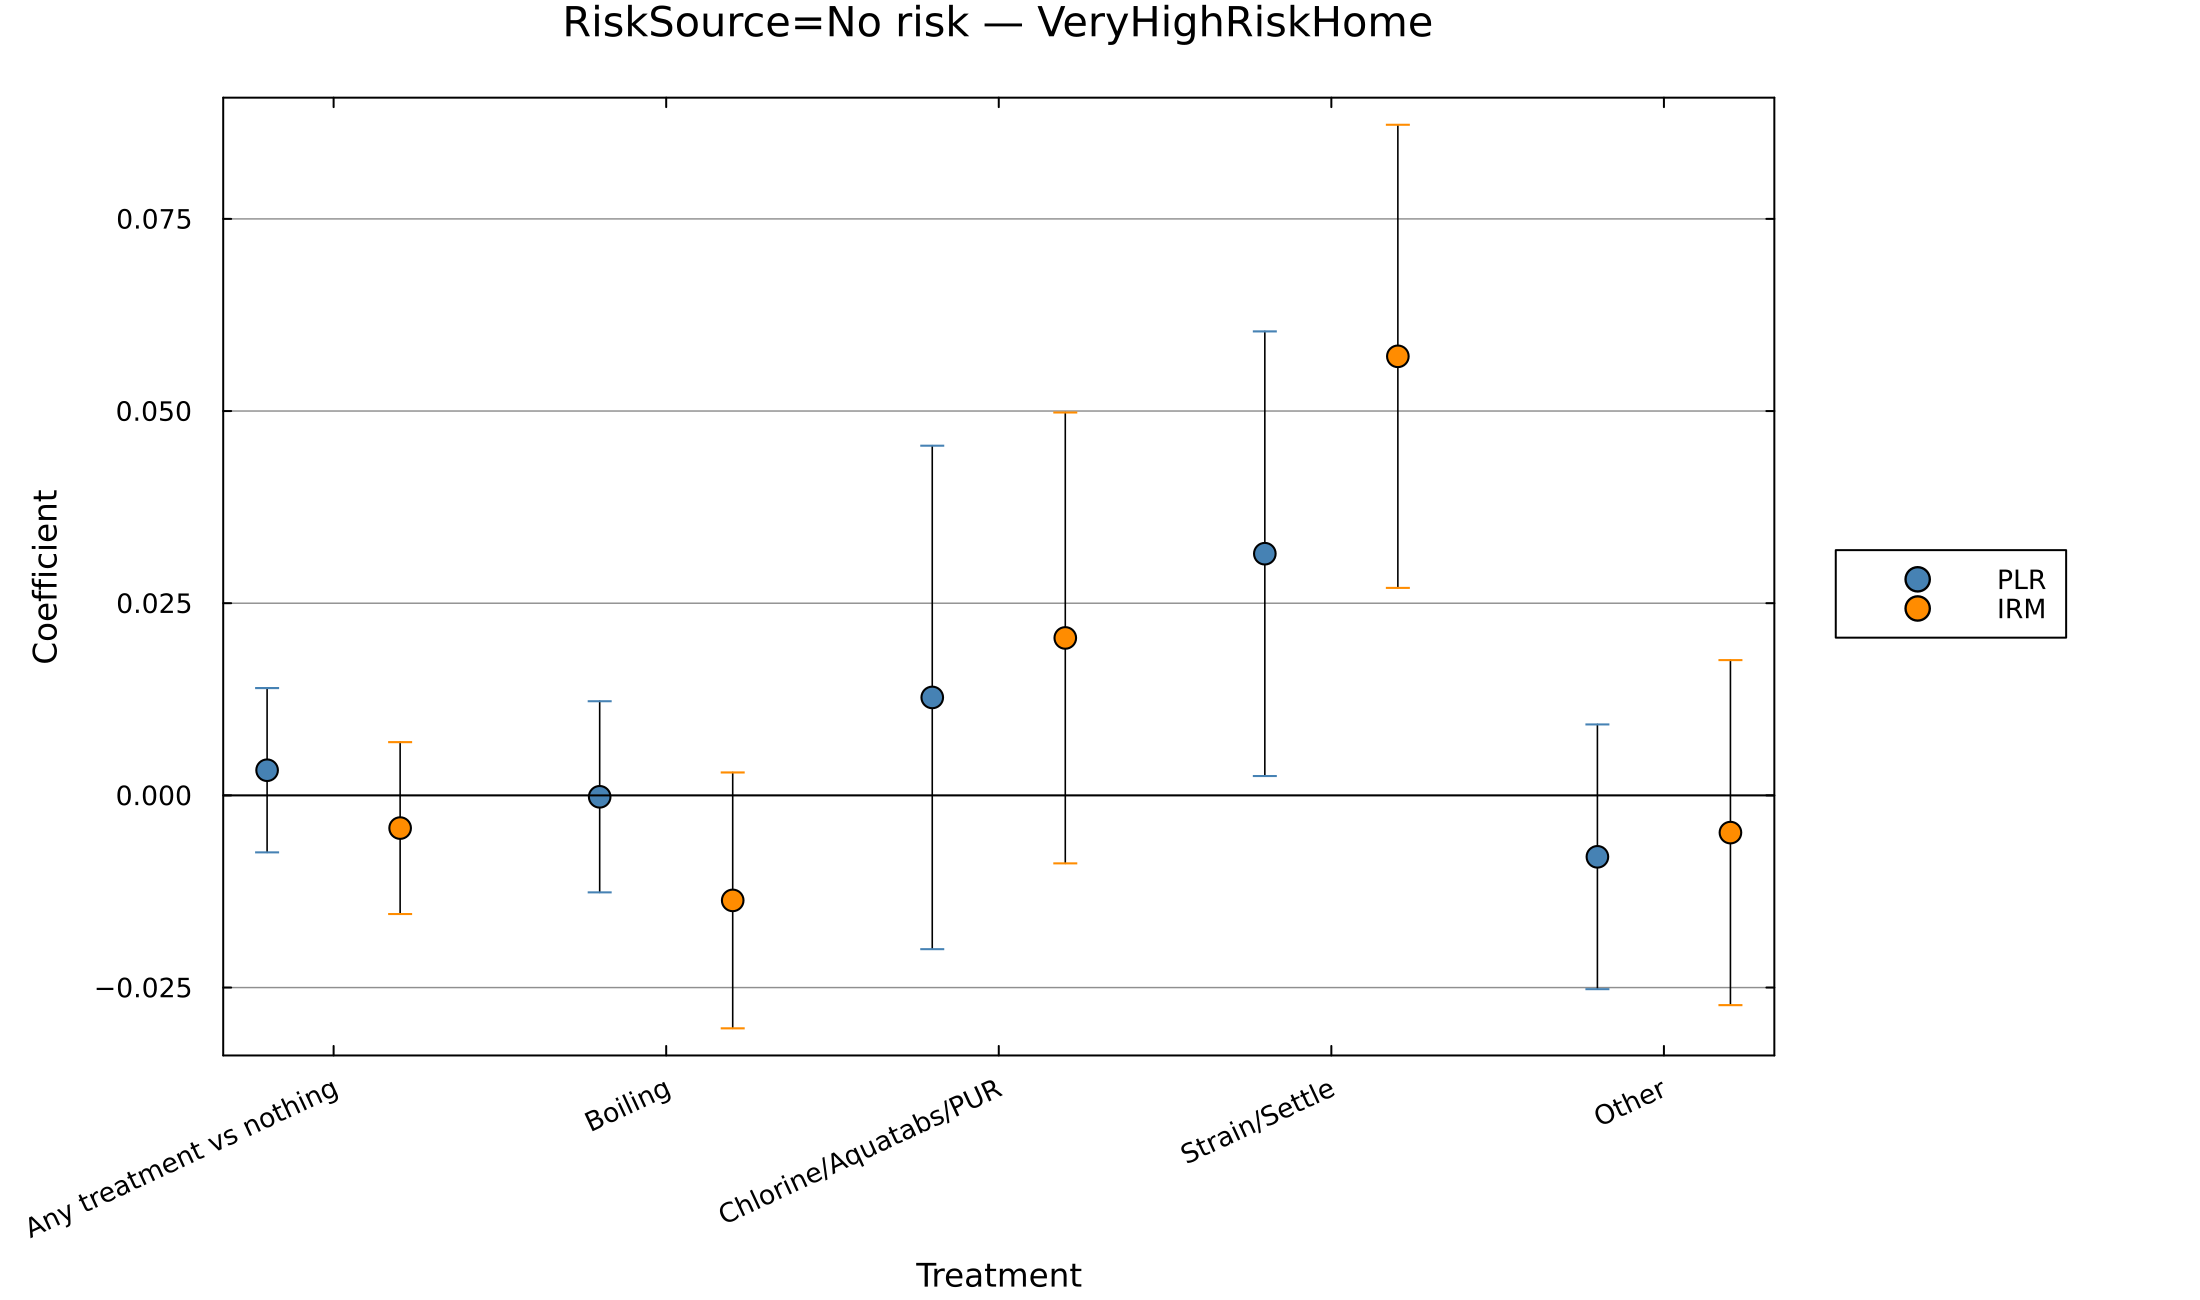
\includegraphics[width=\textwidth]{coefplot_Treatments_RiskSourceNo_risk_VeryHighRiskHome_PLR_IRM.png}\end{subfigure}
%\begin{subfigure}[b]{0.7\textwidth}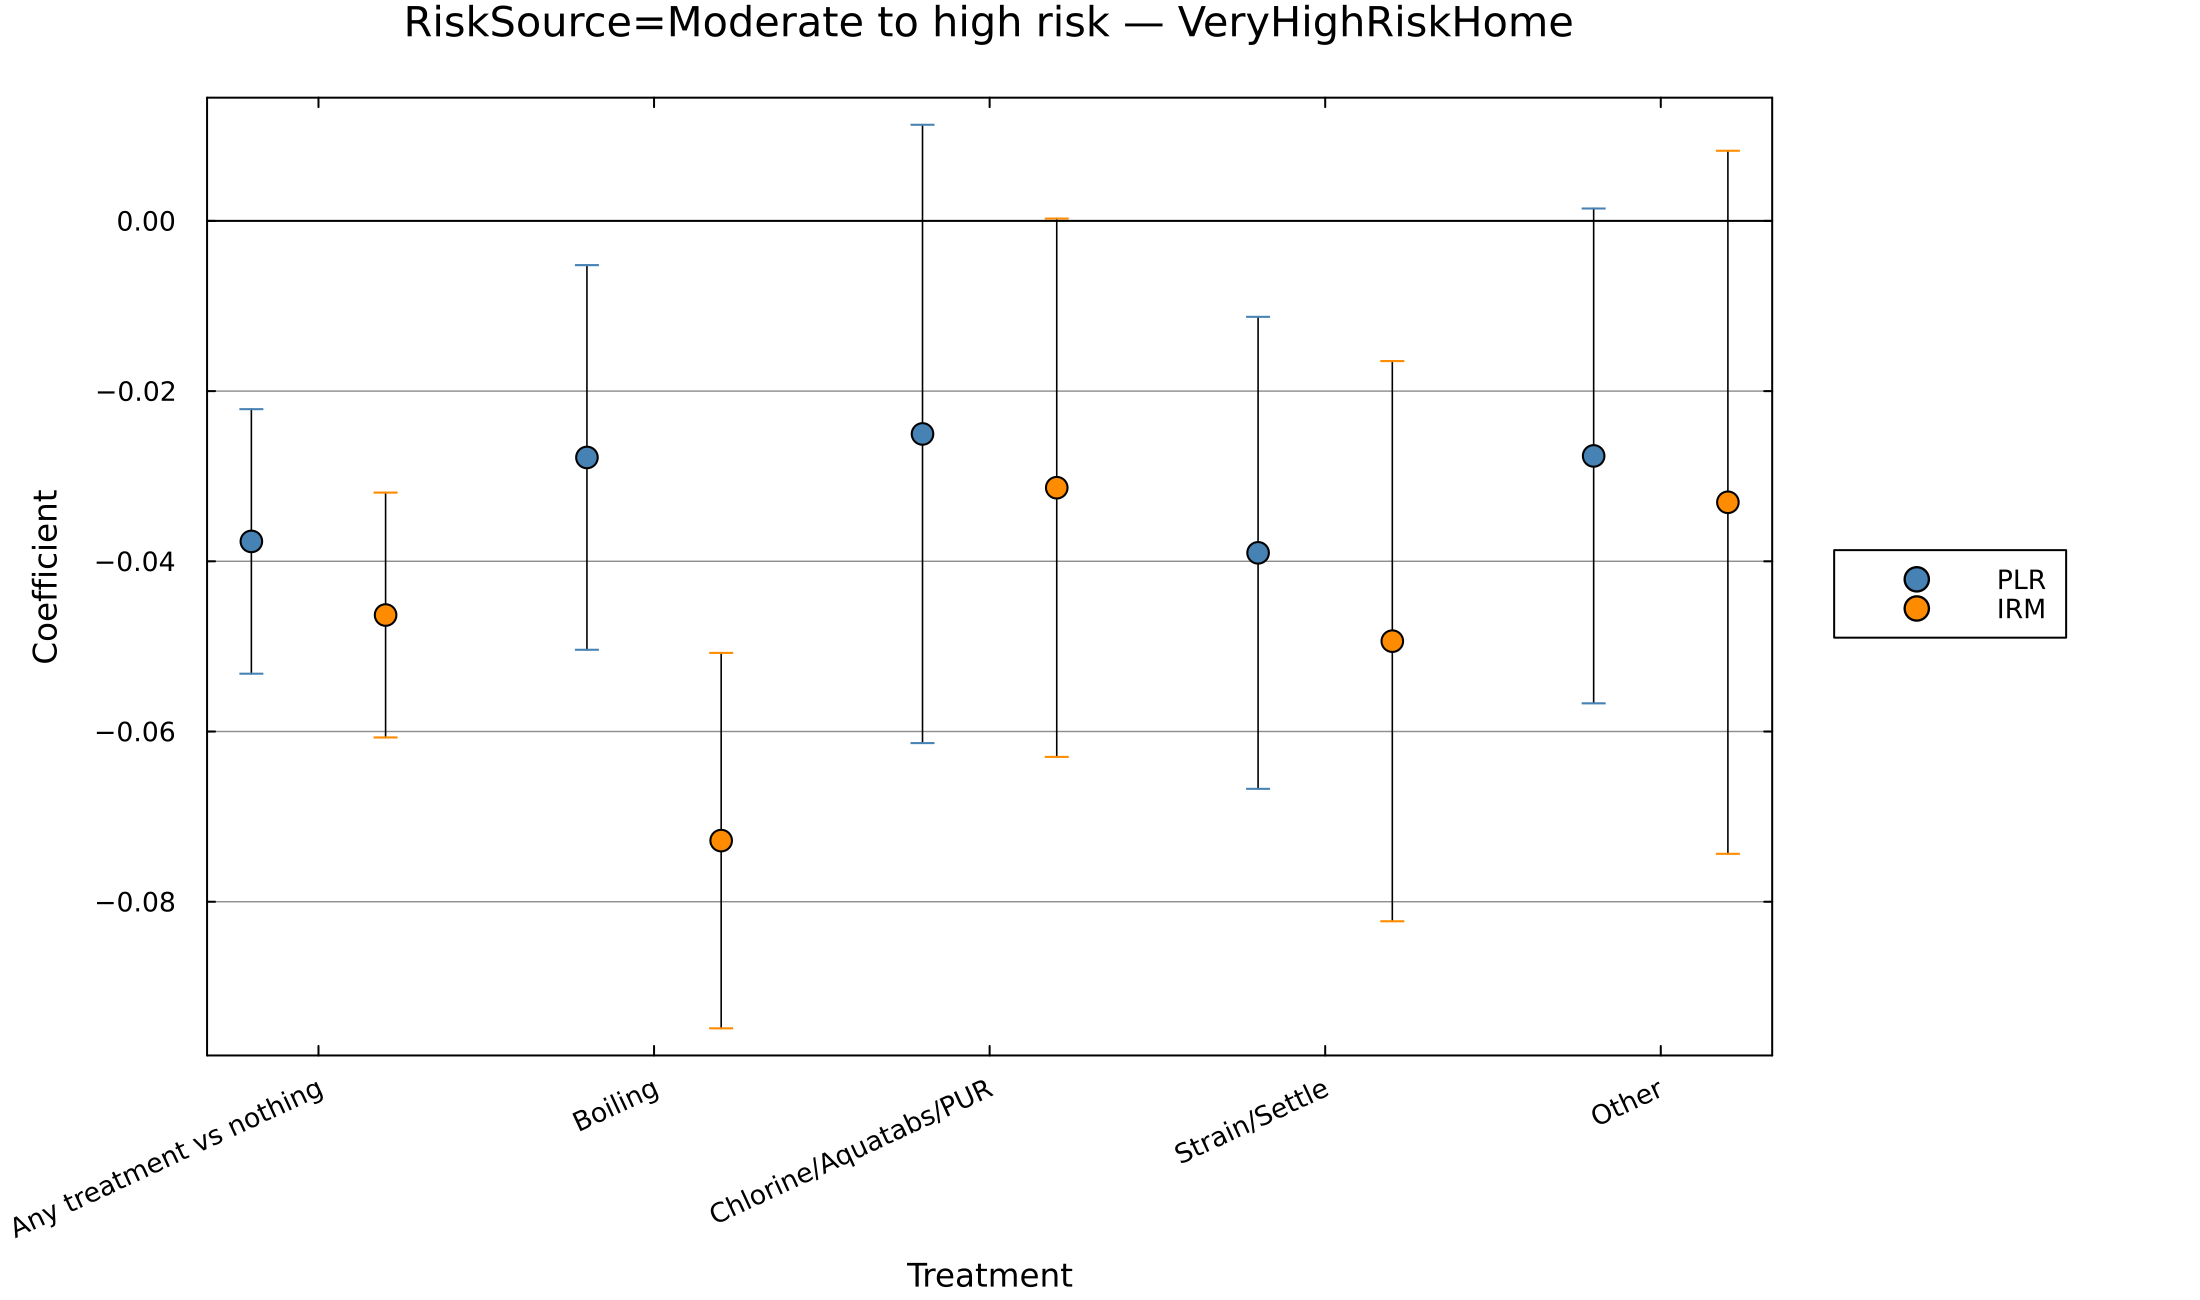
\includegraphics[width=\textwidth]{coefplot_Treatments_RiskSourceModerate_to_high_risk_VeryHighRiskHome_PLR_IRM.png}\end{subfigure}
%\begin{subfigure}[b]{0.7\textwidth}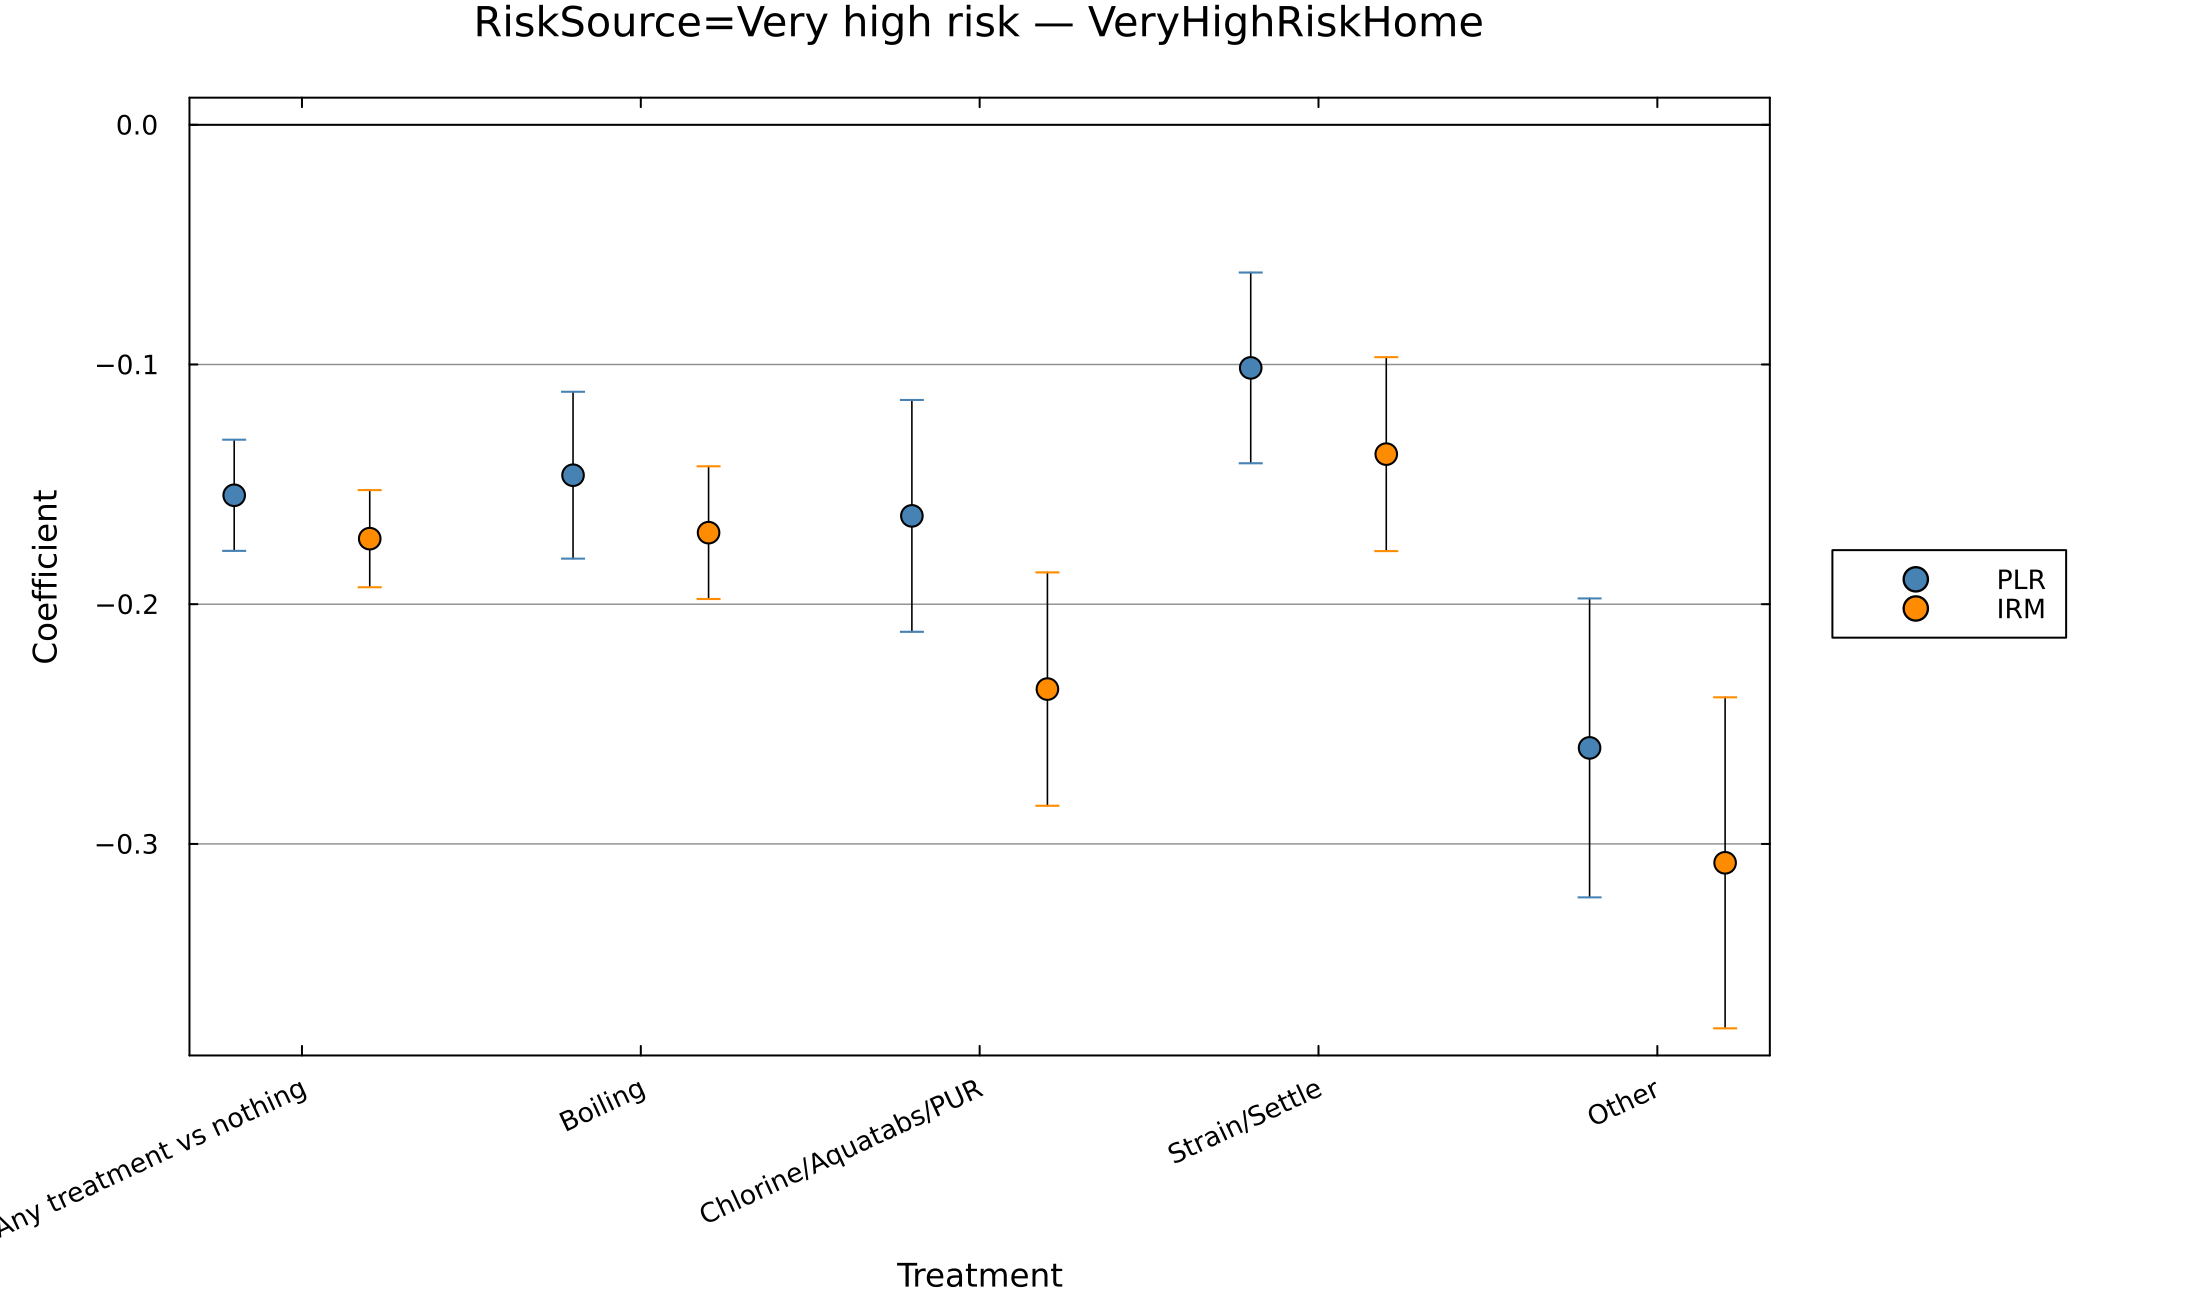
\includegraphics[width=\textwidth]{coefplot_Treatments_RiskSourceVery_high_risk_VeryHighRiskHome_PLR_IRM.png}\end{subfigure}
{\footnotesize  \begin{flushleft} Notes: .\end{flushleft}}
\end{figure}







%========================================================
% TABLE: Benchmark effects, OLS vs PLM vs Interactive
%========================================================

\begin{table}[htbp]\centering
\caption{Effect of Household Water Treatment on E.coli Risk: OLS, PLM, and IRM DDML}
\label{tab:benchmark_main}
\begin{tabular}{lcccccc}
\toprule \toprule
& \multicolumn{3}{c}{SomeRiskHome} & \multicolumn{3}{c}{VeryHighRiskHome} \\
\cmidrule(lr){2-4} \cmidrule(lr){5-7}
& OLS & PLM & IRM & OLS & PLM & IRM \\
\midrule
\multicolumn{7}{l}{\textbf{Panel A: Base controls}} \\
\midrule
HWT ($D$) &
$-0.074^{***}$ & $-0.072^{***}$ & $-0.073^{***}$ &
$-0.050^{***}$ & $-0.057^{***}$ & $-0.058^{***}$ \\
& $(0.005)$ & $(0.005)$ & $(0.005)$ & $(0.006)$ & $(0.006)$ & $(0.006)$ \\
Observations &
56{,}721 & 56{,}721 & 56{,}721 & 56{,}721 & 56{,}721 & 56{,}721 \\
\midrule
\multicolumn{7}{l}{\textbf{Panel B: Extended controls}} \\
\midrule
HWT ($D$) &
$-0.071^{***}$ & $-0.065^{***}$ & $-0.066^{***}$ &
$-0.046^{***}$ & $-0.050^{***}$ & $-0.050^{***}$ \\
& $(0.005)$ & $(0.005)$ & $(0.005)$ & $(0.006)$ & $(0.006)$ & $(0.006)$ \\
Observations &
55{,}510 & 55{,}510 & 55{,}510 & 55{,}510 & 55{,}510 & 55{,}510 \\
\bottomrule \bottomrule
\end{tabular}
\begin{flushleft}
\footnotesize
Notes: Entries report coefficients on the household water treatment indicator from OLS linear probability models, DDML partially linear model (PLM) estimators, and DDML interactive (IRM) estimators using stacked machine learning. All specifications include country fixed effects and the indicated sets of controls. Robust standard errors in parentheses. $^{*} p<0.10$, $^{**} p<0.05$, $^{***} p<0.01$.
\end{flushleft}
\end{table}


%========================================================
% TABLE: Heterogeneity by source risk
%========================================================

\begin{table}[htbp]\centering
\caption{Effect of Household Water Treatment on E.coli Risk, by Source Contamination: OLS, PLM, and IRM DDML}
\label{tab:risk_main}
\begin{tabular}{lcccccc}
\toprule \toprule
& \multicolumn{3}{c}{SomeRiskHome} & \multicolumn{3}{c}{VeryHighRiskHome} \\
\cmidrule(lr){2-4} \cmidrule(lr){5-7}
& OLS & PLM & IRM & OLS & PLM & IRM \\
\midrule
\multicolumn{7}{l}{\textbf{Panel A: RiskSource = 0 (low risk source)}} \\
\midrule
HWT ($D$) &
$-0.077^{***}$ & $-0.067^{***}$ & $-0.068^{***}$ &
$-0.003$ & $-0.005$ & $-0.006$ \\
& $(0.010)$ & $(0.010)$ & $(0.010)$ & $(0.007)$ & $(0.007)$ & $(0.007)$ \\
Observations &
23{,}595 & 23{,}595 & 23{,}595 & 23{,}595 & 23{,}595 & 23{,}595 \\
\midrule
\multicolumn{7}{l}{\textbf{Panel B: RiskSource = 1 (moderate risk source)}} \\
\midrule
HWT ($D$) &
$-0.123^{***}$ & $-0.115^{***}$ & $-0.117^{***}$ &
$-0.049^{***}$ & $-0.041^{***}$ & $-0.043^{***}$ \\
& $(0.006)$ & $(0.006)$ & $(0.006)$ & $(0.009)$ & $(0.009)$ & $(0.009)$ \\
Observations &
21{,}064 & 21{,}064 & 21{,}064 & 21{,}064 & 21{,}064 & 21{,}064 \\
\midrule
\multicolumn{7}{l}{\textbf{Panel C: RiskSource = 2 (very high risk source)}} \\
\midrule
HWT ($D$) &
$-0.090^{***}$ & $-0.084^{***}$ & $-0.086^{***}$ &
$-0.218^{***}$ & $-0.217^{***}$ & $-0.219^{***}$ \\
& $(0.005)$ & $(0.005)$ & $(0.005)$ & $(0.010)$ & $(0.010)$ & $(0.010)$ \\
Observations &
12{,}062 & 12{,}062 & 12{,}062 & 12{,}062 & 12{,}062 & 12{,}062 \\
\bottomrule \bottomrule
\end{tabular}
\begin{flushleft}
\footnotesize
Notes: Entries report coefficients on the household water treatment indicator from OLS linear probability models, DDML PLM estimators, and DDML interactive estimators using stacked machine learning, with base controls. RiskSource is defined by \emph{E.~coli} counts in the household's source water sample: 0 CFU (low risk), 1--100 CFU (moderate risk), and $>$ 100 CFU per 100 mL (very high risk). All specifications include country fixed effects. Robust standard errors in parentheses. $^{*} p<0.10$, $^{**} p<0.05$, $^{***} p<0.01$.
\end{flushleft}
\end{table}



\begin{landscape}
%\begin{table}[htbp]\centering
\caption{Effect of Household Water Treatment on E.coli Risk (SomeRiskHome)}
\newcommand{\sym}[1]{\ifmmode^{#1}\else\(^{#1}\)\fi}
\begin{tabular}{l*{8}{c}}
\toprule
            &\multicolumn{1}{c}{(1)}&\multicolumn{1}{c}{(2)}&\multicolumn{1}{c}{(3)}&\multicolumn{1}{c}{(4)}&\multicolumn{1}{c}{(5)}&\multicolumn{1}{c}{(6)}&\multicolumn{1}{c}{(7)}&\multicolumn{1}{c}{(8)}\\
            &\multicolumn{1}{c}{OLS (LPM)}&\multicolumn{1}{c}{Logit}&\multicolumn{1}{c}{Lasso}&\multicolumn{1}{c}{Ridge}&\multicolumn{1}{c}{Elastic net}&\multicolumn{1}{c}{Random forest}&\multicolumn{1}{c}{Gradient boost}&\multicolumn{1}{c}{Best (stacked)}\\
\multicolumn{9}{l}{\textbf{Panel A: Base controls}}\\
\midrule
water\_treatment&      -0.074\sym{***}&      -0.062\sym{***}&      -0.065\sym{***}&      -0.065\sym{***}&      -0.065\sym{***}&      -0.072\sym{***}&      -0.066\sym{***}&      -0.072\sym{***}\\
            &     (0.005)         &     (0.005)         &     (0.005)         &     (0.005)         &     (0.005)         &     (0.005)         &     (0.005)         &     (0.005)         \\
\midrule
Observations&      56,721         &      56,721         &      56,721         &      56,721         &      56,721         &      56,721         &      56,721         &      56,721         \\

\midrule
\multicolumn{9}{l}{\textbf{Panel B: Extended controls}}\\
\midrule

water\_treatment&      -0.071\sym{***}&      -0.060\sym{***}&      -0.064\sym{***}&      -0.062\sym{***}&      -0.064\sym{***}&      -0.072\sym{***}&      -0.061\sym{***}&      -0.065\sym{***}\\
            &     (0.005)         &     (0.005)         &     (0.005)         &     (0.005)         &     (0.005)         &     (0.005)         &     (0.005)         &     (0.005)         \\
\midrule
Observations&      55,510         &      55,510         &      55,510         &      55,510         &      55,510         &      55,510         &      55,510         &      55,510         \\
\bottomrule\end{tabular}\end{table}
\label{SR_plm}
\end{landscape}

\begin{landscape}
%\begin{table}[htbp]\centering
\caption{Effect of Household Water Treatment on Very High E.coli Risk (VeryHighRiskHome)}
\newcommand{\sym}[1]{\ifmmode^{#1}\else\(^{#1}\)\fi}
\begin{tabular}{l*{8}{c}}
\toprule
            &\multicolumn{1}{c}{(1)}&\multicolumn{1}{c}{(2)}&\multicolumn{1}{c}{(3)}&\multicolumn{1}{c}{(4)}&\multicolumn{1}{c}{(5)}&\multicolumn{1}{c}{(6)}&\multicolumn{1}{c}{(7)}&\multicolumn{1}{c}{(8)}\\
            &\multicolumn{1}{c}{OLS (LPM)}&\multicolumn{1}{c}{Logit}&\multicolumn{1}{c}{Lasso}&\multicolumn{1}{c}{Ridge}&\multicolumn{1}{c}{Elastic net}&\multicolumn{1}{c}{Random forest}&\multicolumn{1}{c}{Gradient boost}&\multicolumn{1}{c}{Best (stacked)}\\
\multicolumn{9}{l}{\textbf{Panel A: Base controls}}\\
\midrule
water\_treatment&      -0.050\sym{***}&      -0.041\sym{***}&      -0.044\sym{***}&      -0.045\sym{***}&      -0.044\sym{***}&      -0.062\sym{***}&      -0.053\sym{***}&      -0.057\sym{***}\\
            &     (0.006)         &     (0.006)         &     (0.006)         &     (0.006)         &     (0.006)         &     (0.006)         &     (0.006)         &     (0.006)         \\
\midrule
Observations&      56,721         &      56,721         &      56,721         &      56,721         &      56,721         &      56,721         &      56,721         &      56,721         \\

\midrule
\multicolumn{9}{l}{\textbf{Panel B: Extended controls}}\\
\midrule

water\_treatment&      -0.046\sym{***}&      -0.039\sym{***}&      -0.042\sym{***}&      -0.039\sym{***}&      -0.041\sym{***}&      -0.057\sym{***}&      -0.046\sym{***}&      -0.050\sym{***}\\
            &     (0.006)         &     (0.006)         &     (0.006)         &     (0.006)         &     (0.006)         &     (0.006)         &     (0.006)         &     (0.006)         \\
\midrule
Observations&      55,510         &      55,510         &      55,510         &      55,510         &      55,510         &      55,510         &      55,510         &      55,510         \\
\bottomrule\end{tabular}\end{table}
\label{VH_plm}
\end{landscape}


\clearpage
\section{Diarrhea and fever}
%-------------------------------------------------------------%
{\renewcommand\normalsize{\small}\normalsize\singlespacing  
\begin{table}[!ht]\centering
\caption{OLS Estimates for Probability of under 5 children having diarrhea}\label{tab:Est_OLS_diarrhea_full}
\begin{tabular}{l}
\hline \hline
\textbf{Panel A: No controls}\\[2pt]
{
\def\sym#1{\ifmmode^{#1}\else\(^{#1}\)\fi}
\begin{tabular}{l*{8}{c}}
\hline\hline
                    &\multicolumn{2}{c}{Across}                 &\multicolumn{2}{c}{Low risk at source}     &\multicolumn{2}{c}{Medium risk at source}  &\multicolumn{2}{c}{High risk at source}    \\\cmidrule(lr){2-3}\cmidrule(lr){4-5}\cmidrule(lr){6-7}\cmidrule(lr){8-9}
                    &\multicolumn{1}{c}{(1)}         &\multicolumn{1}{c}{(2)}         &\multicolumn{1}{c}{(3)}         &\multicolumn{1}{c}{(4)}         &\multicolumn{1}{c}{(5)}         &\multicolumn{1}{c}{(6)}         &\multicolumn{1}{c}{(7)}         &\multicolumn{1}{c}{(8)}         \\
\hline
Any treatment &                     &      -0.035\sym{***}&                     &      -0.042\sym{***}&                     &      -0.030\sym{***}&                     &      -0.031\sym{***}\\
                    &                     &     (0.005)         &                     &     (0.007)         &                     &     (0.008)         &                     &     (0.009)         \\
Boiling             &      -0.050\sym{***}&                     &      -0.052\sym{***}&                     &      -0.048\sym{***}&                     &      -0.046\sym{***}&                     \\
                    &     (0.006)         &                     &     (0.009)         &                     &     (0.011)         &                     &     (0.013)         &                     \\
Chlorination        &      -0.006         &                     &       0.003         &                     &      -0.004         &                     &      -0.016         &                     \\
                    &     (0.013)         &                     &     (0.026)         &                     &     (0.022)         &                     &     (0.021)         &                     \\
Strain              &      -0.015\sym{*}  &                     &      -0.023         &                     &       0.000         &                     &      -0.027\sym{**} &                     \\
                    &     (0.008)         &                     &     (0.015)         &                     &     (0.014)         &                     &     (0.013)         &                     \\
Other treatment     &      -0.067\sym{***}&                     &      -0.063\sym{***}&                     &      -0.097\sym{***}&                     &      -0.015         &                     \\
                    &     (0.009)         &                     &     (0.013)         &                     &     (0.013)         &                     &     (0.028)         &                     \\
male              &       0.008\sym{**} &       0.007\sym{**} &       0.005         &       0.005         &       0.016\sym{***}&       0.016\sym{***}&      -0.001         &      -0.001         \\
                    &     (0.004)         &     (0.004)         &     (0.006)         &     (0.006)         &     (0.006)         &     (0.006)         &     (0.007)         &     (0.007)         \\
Controls            &         Yes         &         Yes         &         Yes         &         Yes         &         Yes         &         Yes         &         Yes         &         Yes         \\
\hline
Mean                &        0.15         &        0.15         &        0.14         &        0.14         &        0.15         &        0.15         &        0.15         &        0.15         \\
Adjusted \(R^{2}\)  &        0.02         &        0.02         &        0.02         &        0.02         &        0.02         &        0.02         &        0.02         &        0.02         \\
Observations        &      36,121         &      36,121         &      12,629         &      12,629         &      13,893         &      13,893         &       9,599         &       9,599         \\
\hline\hline
\end{tabular}
}
\\[6pt]
\textbf{Panel B: Controls}\\[2pt]
{
\def\sym#1{\ifmmode^{#1}\else\(^{#1}\)\fi}
\begin{tabular}{l*{8}{c}}
\hline\hline
                    &\multicolumn{2}{c}{Across}                 &\multicolumn{2}{c}{Low risk at source}     &\multicolumn{2}{c}{Medium risk at source}  &\multicolumn{2}{c}{High risk at source}    \\\cmidrule(lr){2-3}\cmidrule(lr){4-5}\cmidrule(lr){6-7}\cmidrule(lr){8-9}
                    &\multicolumn{1}{c}{(1)}         &\multicolumn{1}{c}{(2)}         &\multicolumn{1}{c}{(3)}         &\multicolumn{1}{c}{(4)}         &\multicolumn{1}{c}{(5)}         &\multicolumn{1}{c}{(6)}         &\multicolumn{1}{c}{(7)}         &\multicolumn{1}{c}{(8)}         \\
\hline
Any treatment &                     &      -0.000         &                     &       0.010         &                     &      -0.000         &                     &      -0.010         \\
                    &                     &     (0.006)         &                     &     (0.011)         &                     &     (0.010)         &                     &     (0.011)         \\
Boiling             &       0.005         &                     &       0.011         &                     &      -0.001         &                     &       0.002         &                     \\
                    &     (0.008)         &                     &     (0.014)         &                     &     (0.013)         &                     &     (0.016)         &                     \\
Chlorination        &      -0.015         &                     &      -0.008         &                     &      -0.006         &                     &      -0.037\sym{*}  &                     \\
                    &     (0.013)         &                     &     (0.027)         &                     &     (0.022)         &                     &     (0.021)         &                     \\
Strain              &       0.008         &                     &       0.015         &                     &       0.024         &                     &      -0.009         &                     \\
                    &     (0.011)         &                     &     (0.023)         &                     &     (0.018)         &                     &     (0.020)         &                     \\
Other treatment     &      -0.009         &                     &       0.013         &                     &      -0.046\sym{***}&                     &       0.020         &                     \\
                    &     (0.010)         &                     &     (0.016)         &                     &     (0.014)         &                     &     (0.028)         &                     \\
male              &       0.010\sym{***}&       0.010\sym{***}&       0.008         &       0.008         &       0.017\sym{***}&       0.017\sym{***}&       0.002         &       0.002         \\
                    &     (0.004)         &     (0.004)         &     (0.006)         &     (0.006)         &     (0.006)         &     (0.006)         &     (0.007)         &     (0.007)         \\
Controls            &         Yes         &         Yes         &         Yes         &         Yes         &         Yes         &         Yes         &         Yes         &         Yes         \\
\hline
Mean                &        0.15         &        0.15         &        0.14         &        0.14         &        0.15         &        0.15         &        0.15         &        0.15         \\
Adjusted \(R^{2}\)  &        0.05         &        0.05         &        0.06         &        0.06         &        0.05         &        0.05         &        0.05         &        0.05         \\
Observations        &      36,121         &      36,121         &      12,629         &      12,629         &      13,893         &      13,893         &       9,599         &       9,599         \\
\hline\hline
\end{tabular}
}
\\[4pt]
\multicolumn{1}{p{0.95\linewidth}}{Notes: $\sym{*} p<0.10,\sym{**} p<0.05,\sym{***} p<0.01$.} \\
\hline
\end{tabular}
\end{table}

}  
%-------------------------------------------------------------% 

%-------------------------------------------------------------%
{\renewcommand\normalsize{\small}\normalsize\singlespacing  
\input{Table/Est_OLS_fever_full.tex}
}  
%-------------------------------------------------------------% 

% We estimate the causal effect of household water treatment on E. coli contamination using the DDML framework with XGBoost for nuisance function estimation (see Appendix Table~\ref{tab:robustness_comparison} for model performance). We present both PLR and IRM estimates, where convergence indicates linear effects and divergence suggests non-linearities.

% Tables~\ref{tab:somerisk_base} and~\ref{tab:somerisk_ext} present treatment effects on any E. coli contamination (SomeRiskHome). Both specifications show significant negative effects.

% The base model shows treatment reduces contamination by 5.3--7.1 percentage points (IRM: $-0.0529$; PLR: $-0.0708$). Extended models, which include household composition, sanitation infrastructure, and detailed water service characteristics, show larger effects of 7.7--8.6 percentage points (IRM: $-0.0774$; PLR: $-0.0864$). The 0.9 percentage point convergence between PLR and IRM in the extended specification indicates treatment effects are largely linear once comprehensive controls are included.

% Tables~\ref{tab:veryhigh_base} and~\ref{tab:veryhigh_ext} present effects on severe contamination (VeryHighRiskHome).

% Treatment reduces severe contamination by 4.7--5.3 percentage points in base models and 6.5 percentage points in extended models (IRM: $-0.0645$; PLR: $-0.0652$). The near-perfect convergence (0.07 percentage points) between PLR and IRM indicates treatment operates linearly on severe contamination.

% Stratifying by water source risk reveals important heterogeneity. Tables~\ref{tab:somerisk_no_risk}, \ref{tab:somerisk_moderate_to_high_risk}, and~\ref{tab:somerisk_very_high_risk} show SomeRiskHome effects by risk category.

% Treatment effects are largest for moderate to high risk sources (9.9--11.5 percentage points), compared to very high risk (6.5--8.4 percentage points) and no-risk sources (6.0--6.8 percentage points). This inverted U-shaped pattern suggests households with moderate contamination benefit most—their water quality is poor enough to benefit from treatment but not so severe that point-of-use treatment is overwhelmed. Very high risk sources may indicate broader environmental contamination that household treatment alone cannot fully address.

% Tables~\ref{tab:veryhigh_no_risk}, \ref{tab:veryhigh_moderate_to_high_risk}, and~\ref{tab:veryhigh_very_high_risk} show VeryHighRiskHome effects by risk category.

% The pattern for severe contamination differs markedly. No-risk sources show no significant effects, consistent with these sources rarely producing severe contamination. Moderate to high risk sources show effects of 3.2--4.7 percentage points. The largest effects emerge for very high risk sources: treatment reduces severe contamination by 21.0--21.9 percentage points. This dramatic reduction indicates that even when water sources are severely contaminated, point-of-use treatment effectively prevents the most dangerous contamination events. PLR and IRM estimates converge across all subsamples (differences $<$ 0.6 percentage points), confirming linear treatment effects.

% The extended model consistently produces larger effects than the base model (1.3--2.5 percentage points), indicating that household and infrastructure controls reduce omitted variable bias. The heterogeneity patterns are theoretically coherent: moderate risk sources show the largest effects for any contamination, while very high risk sources show the largest effects for severe contamination, reflecting different mechanisms of treatment effectiveness across the contamination distribution.

\iffalse
%-------------------------------------------------------------%
{\renewcommand\normalsize{}\normalsize\singlespacing  
\input{Table/ddml_partial_SomeEcoli_bi_full.tex}
\begin{table}[htbp]\centering
\def\sym#1{\ifmmode^{#1}\else\(^{#1}\)\fi}
\caption{Diarrhea: OLS vs. DDML (LASSO / RF) and BEST — Partial Effect of $D$ on $Y$}
\begin{tabular}{l*{1}{c}}
\toprule
                &\multicolumn{1}{c}{(1)}\\
                &\multicolumn{1}{c}{OLS}\\
\midrule
Any treatment (Water tested)&   -0.084\sym{***}\\
                &  (0.016)         \\
\midrule
Observations    &   19,562         \\
Reps            &        5         \\
D\_water\_treatment\_ss\_mse&                  \\
Y\_SomeRiskHome\_ss1\_mse&                  \\
Y\_SomeRiskHome\_ss0\_mse&                  \\
\bottomrule
\end{tabular}
\end{table}

\input{Table/ddml_partial_Ecoli_bi_full.tex}
\input{Table/ddml_interactive_Ecoli_bi_full.tex}
\begin{table}[htbp]\centering
\def\sym#1{\ifmmode^{#1}\else\(^{#1}\)\fi}
\caption{Diarrhea: OLS vs. DDML (LASSO / RF) and BEST — Partial Effect of $D$ on $Y$}
\begin{tabular}{l*{1}{c}}
\toprule
                &\multicolumn{1}{c}{(1)}\\
                &\multicolumn{1}{c}{OLS}\\
\midrule
Any treatment (Water tested)&   -0.016         \\
                &  (0.016)         \\
\midrule
Observations    &   14,130         \\
Reps            &        5         \\
D\_water\_treatment\_ss\_mse&                  \\
Y\_diarrhea\_ss\_mse&                  \\
\bottomrule
\end{tabular}
\end{table}

\begin{table}[htbp]\centering
\def\sym#1{\ifmmode^{#1}\else\(^{#1}\)\fi}
\caption{Diarrhea: OLS vs. DDML (LASSO / RF) and BEST — Partial Effect of $D$ on $Y$}
\begin{tabular}{l*{1}{c}}
\toprule
                &\multicolumn{1}{c}{(1)}\\
                &\multicolumn{1}{c}{OLS}\\
\midrule
Any treatment (Water tested)&   -0.025         \\
                &  (0.020)         \\
\midrule
Observations    &   14,130         \\
Reps            &        5         \\
D\_water\_treatment\_ss\_mse&                  \\
Y\_diarrhea\_ss1\_mse&                  \\
Y\_diarrhea\_ss0\_mse&                  \\
\bottomrule
\end{tabular}
\end{table}

}  
%-------------------------------------------------------------% 
\fi

\section{Conclusion}  

The Lancet Commission on water, sanitation, and hygiene highlights the urgent need for investments in WASH services, particularly in low- and middle-income countries, to reduce health disparities. Access to safe drinking water is critical in preventing infectious diseases, including those caused by E. Coli contamination \cite{lancet2021commission}. 
%Another study provides updated estimates on the impact of water, sanitation, and hygiene (WASH) interventions on childhood diarrhoea in low- and middle-income countries (LMICs). It demonstrates that interventions such as water treatment at the point of use, improved drinking water sources, sanitation with sewer connections, and handwashing with soap can significantly reduce the risk of diarrhoea in children \cite{wolf2022effectiveness}. These findings highlight the crucial role of WASH interventions in mitigating diarrhoeal disease, although no studies evaluated interventions achieving universal access to safely managed WASH services. The Lancet Commission on water, sanitation, hygiene, and health highlights the critical importance of improving WASH services for controlling diarrheal diseases, particularly those caused by E. Coli contamination in water. Water treatment interventions should focus not only on microbiological water quality but also address a broader spectrum of health outcomes beyond diarrhea, including mental health and gender disparities \cite{stoler2023revisiting}.


\subsection*{Contributors}  

\subsection*{Declaration of interests}  
All authors declare no competing interests.

\subsection*{Data sharing}  
All data used for this and analytical codes are available immediately following publication without an end date to anyone for any purpose and are either published in the appendices or can be accessed through the corresponding author.

\subsection*{Acknowledgments}  

\clearpage 
% \nocite{*}
\bibliographystyle{apacite}
\bibliography{Citation_Water}



\clearpage   
%%%%%%%     
% Appendix %
%%%%%%%
\renewcommand\thefigure{\thesection.\arabic{figure}}   
\renewcommand\thetable{\thesection.\arabic{table}}   


\clearpage
\doublespacing  
\begin{appendices}
\section{Sample}\label{Sample0}\setcounter{figure}{0}\setcounter{table}{0}
Table \ref{SurNum} reports the total number of households in the full survey, the number selected for the water quality testing module, and the number that provided consent. It also shows the number of samples with missing values for either water source or stored drinking water quality data, the number of samples missing water treatment information, and the final number of samples included in the analysis.

%-------------------------------------------------------------%
{\renewcommand\normalsize{\footnotesize}\normalsize\singlespacing  
\begin{table}[htbp] \centering
\caption{Number of Household Surveys and Sample Included in the Analysis}
\label{SurNum}
\newcolumntype{P}[1]{>{\centering\arraybackslash}p{#1}}
\begin{tabular}{l P{1.2cm} | P{1.2cm} P{1.5cm} | P{1.2cm} P{2cm} P{2.2cm} | P{1.2cm} P{1.2cm}}
&\textbf{Total}& \multicolumn{2}{c}{\textbf{Selected}} & \multicolumn{3}{c}{\textbf{Not in the sample (N)}} & \multicolumn{2}{c}{\textbf{Complete}} \\
& N & N & (\%) & No consent & Water test missing & Water treatment missing & N & (\%) \\
\textbf{Sub-Saharan Africa} &&&&&&& \\ \hline


Central African Rep&8,133&1,228&15.1&3&188&1&1,036&84.4 \tabularnewline
Chad&18,967&2,284&12&0&171&0&2,113&92.5 \tabularnewline
Gambia&7,405&1,879&25.4&14&113&1&1,751&93.2 \tabularnewline
Zimbabwe&11,091&2,138&19.3&8&136&2&1,992&93.2 \tabularnewline
Togo&7,916&1,157&14.6&0&73&2&1,082&93.5 \tabularnewline
Eswatini&4,675&1,235&26.4&8&63&4&1,160&93.9 \tabularnewline
Madagascar&17,870&3,439&19.2&6&169&4&3,260&94.8 \tabularnewline
Benin&16,790&3,809&22.7&10&142&8&3,649&95.8 \tabularnewline
Lesotho&8,847&1,376&15.6&1&43&0&1,332&96.8 \tabularnewline
Ghana&12,939&3,230&25&3&93&3&3,131&96.9 \tabularnewline
Malawi&25,419&3,208&12.6&9&78&5&3,116&97.1 \tabularnewline
DR Congo&20,792&2,783&13.4&1&76&0&2,706&97.2 \tabularnewline
Sierra Leone&15,309&1,784&11.7&1&36&4&1,743&97.7 \tabularnewline
Guinea Bissau&7,379&1,829&24.8&1&5&1&1,822&99.6 \tabularnewline

 
\textbf{Latin America} &&&&&&& \\ \hline


Honduras&20,669&5,111&24.7&78&1,010&2&4,021&78.7 \tabularnewline
Dominican Republic&31,488&3,125&9.9&81&500&3&2,541&81.3 \tabularnewline
Suriname&7,915&1,982&25&281&83&2&1,616&81.5 \tabularnewline
Guyana&7,072&1,670&23.6&65&206&6&1,393&83.4 \tabularnewline
Trinidad and Tobago&7,499&1,905&25.4&36&265&3&1,601&84 \tabularnewline
Fiji&5,467&1,104&20.2&1&17&0&1,086&98.4 \tabularnewline

 
\textbf{Asia}  &&&&&&& \\ \hline


Mongolia&13,798&2,764&20&19&169&4&2,572&93.1 \tabularnewline
Nepal&12,655&2,547&20.1&1&153&12&2,381&93.5 \tabularnewline
Lao&22,287&3,360&15.1&5&107&0&3,248&96.7 \tabularnewline
Viet Nam&13,359&3,323&24.9&11&79&2&3,231&97.2 \tabularnewline
Bangladesh&61,242&6,152&10&10&90&2&6,050&98.3 \tabularnewline

 \\\hline


\textbf{Total}&386,983&64,422&16.6&653&4,065&71&59,633&92.6 \tabularnewline

\\ 
\multicolumn{9}{p{0.98\linewidth}}{Notes: Households that did not consent to the full survey are excluded from the sample, as household characteristics are unavailable for analysis. Cases with missing water test data reflect instances where water testing was not conducted—either because the household could not provide a water sample, the test was only partially completed, or there were errors in reading the results.}
\end{tabular}
\end{table}
}
%-------------------------------------------------------------% 


\clearpage
\section{Theoretical}\label{DDMLTheo}\setcounter{figure}{0}\setcounter{table}{0}

\begin{definition}[Neyman orthogonality]
In DDML we work with a score $\varphi(W; \theta, \eta)$, where $\theta$ is the low-dimensional parameter of interest (ATE, PLM slope, etc.) and $\eta$ is a (possibly high-dimensional/nonparametric) nuisance object such as regression or propensity functions \citep[Section 2]{chernozhukov2018dml}. Neyman orthogonality requires
\[
\E[\varphi(W; \theta_0, \eta_0)] = 0
\]
and, crucially,
\[
\partial_\eta \,\E[\varphi(W; \theta_0, \eta)]
\big\vert_{\eta = \eta_0} = 0,
\]
i.e.\ the directional derivative with respect to $\eta$ at the truth is zero \citep[Def.~1]{doubleml2022}. This means the population moment is locally insensitive (flat) in the nuisance direction, so if we plug in an estimate $\hat{\eta}$ that is close but not exact, the induced bias in the score is of order $\|\hat{\eta} - \eta_0\|^2$ \citep[Sec.~2.1]{chernozhukov2018dml}.
\end{definition}

\subsection*{Role inside DDML theory}

The DDML theory combines two classic semiparametric ideas: (i) use Neyman-orthogonal scores to kill first-order regularization bias from ML in the first stage, and (ii) use sample-splitting/cross-fitting to kill overfitting bias from using the same data twice \citep[Sec.~2]{chernozhukov2018dml}. Under mild rate conditions---roughly that the ML nuisance estimators converge faster than $n^{-1/4}$ in an appropriate norm---Neyman orthogonality implies that the target estimator $\hat{\theta}$ constructed from the orthogonal score satisfies
\[
\sqrt{n} (\hat{\theta} - \theta_0) \stackrel{d}{\to} N(0, V).
\]

Put differently: in DDML, Neyman orthogonalization is the theoretical device that ``debiases'' plug-in ML, ensuring that as long as the first-stage ML is good enough in aggregate, the remaining bias is negligible relative to $n^{-1/2}$ and valid standard errors and confidence intervals for $\theta$ follow \citep[Sec.~2.2]{doubleml2022}.

\subsection{Partially linear model and orthogonal score}

Consider the partially linear model
\[
Y = \theta_0 D + g_0(X) + U, \quad \E[U \mid X, D] = 0,
\]
with nuisance functions
\[
m_0(X) \coloneqq \E[D \mid X], \quad g_0(X) \coloneqq \E[Y \mid X].
\]
Define the residuals
\[
V \coloneqq D - m(X), \quad R \coloneqq Y - g(X),
\]
where $(g,m)$ are generic candidates for $(g_0,m_0)$.

The Neyman-orthogonal score for $\theta$ in this model is
\[
\varphi(W; \theta, \eta) = (Y - g(X) - \theta (D - m(X)))\,(D - m(X)), \quad W = (Y,D,X), \quad \eta = (g,m),
\]
which coincides with the canonical PLM score used in DDML implementation \citep[Sec.~2]{chernozhukov2018dml,doubleml2022}. At the truth $(\theta_0,\eta_0)$ with $\eta_0 = (g_0,m_0)$,
\[
\E[\varphi(W; \theta_0, \eta_0)] = 0,
\]
so the moment condition identifies $\theta_0$.

Moreover, the score is Neyman-orthogonal in the sense that for any perturbation $(h_g, h_m)$ of $(g_0,m_0)$, the directional derivative
\[
\left. \frac{d}{dt}\,\E\big[\varphi\big(W; \theta_0, (g_0 + t h_g, m_0 + t h_m)\big)\big] \right|_{t=0} = 0.
\]
This can be verified by writing
\[
Y - g_0(X) - \theta_0\bigl(D - m_0(X)\bigr) = U,
\]
and then differentiating inside the expectation and using $\E[U \mid X,D]=0$ together with $\E[D - m_0(X) \mid X]=0$ \citep[Sec.~2]{chernozhukov2018dml}.

This residualization corresponds to the ``partialling out'' interpretation: regress out $X$ from $Y$ and $D$ (estimate $g_0$ and $m_0$), then regress the residual $R$ on $V$ to estimate $\theta_0$ \citep[Fig.~1c]{doubleml2022}. At the population level, this yields
\[
\theta_0 = \frac{\E[(D-m_0(X))(Y-g_0(X))]}{\E[(D-m_0(X))^2]},
\]
which is exactly the PLM coefficient from the regression of $R$ on $V$.

\subsection{Interactive model and doubly robust AIPW score}
\label{sec:theory_irm}

Consider the interactive regression model (IRM) with binary treatment
\[
Y = g_0(D,X) + U,\quad D \in \{0,1\},\quad \E[U \mid X,D] = 0,
\]
where \(g_0(D,X)\) is a fully nonparametric conditional mean function.
Define the nuisance functions
\[
m_0(X) \coloneqq \E[D \mid X] = P(D=1 \mid X),\quad g_{d,0}(X) \coloneqq \E[Y \mid D=d,X],\quad d \in \{0,1\}.
\]

For generic candidates \((g_0,g_1,m)\) for \((g_{0,0},g_{1,0},m_0)\), a natural target parameter is the average treatment effect
\[
\theta_0 \coloneqq \E\bigl[g_{1,0}(X) - g_{0,0}(X)\bigr] = \E[Y^1 - Y^0],
\]
identified under standard unconfoundedness and overlap conditions.

The \emph{Neyman-orthogonal, doubly robust AIPW score} for \(\theta\) in this model is
\[
\varphi(W; \theta, \eta) = \frac{D\,(Y - g_1(X))}{m(X)} - \frac{(1-D)\,(Y - g_0(X))}{1 - m(X)} + g_1(X) - g_0(X) - \theta,
\]
where \(W = (Y,D,X)\) and \(\eta = (g_0,g_1,m)\).
This is the canonical IRM score used in DDML implementations for binary treatment.

At the truth \((\theta_0,\eta_0)\) with \(\eta_0 = (g_{0,0},g_{1,0},m_0)\), the score has mean zero:
\[
\E\bigl[\varphi(W; \theta_0, \eta_0)\bigr] = 0,
\]
so the moment condition identifies \(\theta_0\).

Moreover, the score is \emph{doubly robust} in the sense that
\[
\E\bigl[\varphi(W; \theta_0, (g_0,g_1,m_0))\bigr] = 0 \quad\text{for any } (g_0,g_1),
\]
and
\[
\E\bigl[\varphi(W; \theta_0, (g_{0,0},g_{1,0},m))\bigr] = 0 \quad\text{for any } m,
\]
i.e.\ the moment condition remains valid if either the outcome regressions \((g_0,g_1)\) are correctly specified or the propensity score \(m\) is correctly specified.

In addition, the score is \emph{Neyman-orthogonal} with respect to perturbations of the nuisance functions.
For any directions \((h_{g_0},h_{g_1},h_m)\) in the nuisance space,
\[
\left. \frac{d}{dt}\, \E\Bigl[ \varphi\bigl( W;\theta_0,\bigl(g_{0,0} + t h_{g_0},\, g_{1,0} + t h_{g_1},\, m_0 + t h_m\bigr) \bigr) \Bigr] \right|_{t=0} = 0.
\]
This follows by differentiating inside the expectation and using the identities
\[
\E[Y \mid D=d,X] = g_{d,0}(X),\quad \E[D \mid X] = m_0(X),
\]
together with iterated expectations to show that the first-order effects of perturbations in \((g_0,g_1,m)\) cancel.

At the population level, the AIPW score admits the representation
\[
\theta_0 = \E\left[ \frac{D\,(Y - g_{1,0}(X))}{m_0(X)} - \frac{(1-D)\,(Y - g_{0,0}(X))}{1 - m_0(X)} + g_{1,0}(X) - g_{0,0}(X) \right],
\]
which is exactly the doubly robust augmented inverse probability weighting (AIPW) expression for the average treatment effect in the interactive model.



\clearpage
\section{DDML Command}\setcounter{figure}{0}\setcounter{table}{0}\label{DDMLCommand}
The DDML framework is particularly useful when estimating causal effects in high-dimensional settings, as it allows for flexible machine learning control while preserving valid inference through sample-splitting and orthogonalization.

This section provides guidance on how to use the \texttt{qddml} command, which implements the Double/Debiased Machine Learning (DDML) framework proposed by \citet{chernozhukov2018double}.  
The official documentation can be found at the following link:  
\href{https://statalasso.github.io/docs/ddml/help/}{qddml Help File}.

\bigskip
\noindent
\textbf{Step 1: Set up Python integration in Stata.}  
Before running any DDML commands, you must configure Stata’s Python integration.  
Follow the official setup instructions available here:  
\href{https://statalasso.github.io/docs/python/}{Python Configuration for Stata}.  
This step ensures that DDML can communicate properly with Python-based learners.

\bigskip
\noindent
\textbf{Step 2: Run the analysis do-file.}  
Once Python integration is set up, you can execute the analysis script:  

\href{https://www.youtube.com/watch?v=iiEi-3gIUbg&t=1706s}{Good YouTube video}

\clearpage
\section{E. Coli in drinking water and diarrhea}  

Figure \ref{Count_Morbidity} shows the relationship between E. Coli counts in source and drinking water and the incidence of diarrhea and fever among households. The histograms show the distribution of E. Coli counts in both source and drinking water. The green histogram indicates that the E. Coli count in source water peaks at lower values, while the black histogram shows a similar distribution for drinking water. This distribution indicates that drinking water is more likely to be contaminated than source water, suggesting that water becomes contaminated during storage.

The figure shows that the diarrhea rate is highly correlated with drinking water quality. The average probability of children under age 5 having diarrhea is around 11 percent when the water is not contaminated (E. Coli = 0), but the rate increases to as high as 16 percent if the water is contaminated at levels higher than E. Coli over 100. The contamination level of the water source is unrelated to the prevalence of diarrhea, indicating that households are treating water to reduce E. Coli based on different initial contamination levels. A similar relationship is observed for the incidence of fever.

\begin{figure}[htbp]\centering
\caption{Relationship between E. Coli of Source/Drinking Water and Diarrhea and Fever }\label{Count_Morbidity}
\begin{subfigure}[b]{1\textwidth}\includegraphics[width=\textwidth]{WaterQ_Morbidity.eps}\end{subfigure}
{\footnotesize  \begin{flushleft} Notes: N=22,589 children under age five. The figure shows the relationship between E. Coli counts in source and drinking water and the incidence of diarrhea and fever among households. The histograms show the distribution of E. Coli counts in both source and drinking water.\end{flushleft}}
\end{figure}

\subsection{Water treatment and diarrhea}  
Figure \ref{Desc_0} shows the prevalence of diarrhea among children under age 5, grouped by household water treatment methods. While some countries exhibit a lower prevalence of diarrhea among households that treat their water, the difference is minor. In some instances, the relationship is reversed, with a higher prevalence of diarrhea observed among households that treat their water. Such patterns are widely observed, and several studies using MICS data do not find a clear link between water treatment and diarrhea \citep{husein2023examination}. 

The unclear relationship can be attributed to endogeneity. Households with contaminated water, which is correlated with higher diarrhea prevalence, are more likely to treat their water, while those using uncontaminated water sources are less likely to do so. Another reason for the weak link is the low efficacy of the water treatment itself.

\begin{figure}[htbp]\centering
\caption{Diarrhea prevalence among U5 children by water treatment methods}\label{Desc_0}
\begin{subfigure}[b]{1\textwidth}\includegraphics[width=\textwidth]{Water_Diarrhea_Treat.eps}\end{subfigure}
{\footnotesize  \begin{flushleft} Notes: The prevalence of diarrhea among children under age 5 across 14 countries from MICS, using nationally representative weights. Categories with fewer than 15 samples are excluded from the analysis, as the sample size is too small to calculate a reliable average.\end{flushleft}}
\end{figure}







\section{Notes}

%https://docs.doubleml.org/tutorial/stable/lectures/L1/introduction_part1.html#/neyman-orthogonality-motivation

Why Double Machine Learning?
$$Y=g_0(D,X) + U$$
ML Learner
, $$E(U|X,D)=0$$.
 

Why not simply estimate g0(D,X)
 with ML and plug in predictions $g_0(D,X)$?
ML methods address the variance-bias-tradeoff by introducing some kind of regularization
This will translate into a bias of the causal estimate


Challenges in causal machine learning
Causal estimation after using ML methods for estimation require adjustments of the estimation framework $\implies$ Chernozhukov et al. (2018)


The Key Ingredients of DML
1. Neyman orthogonality
2. High-quality ML estimation
3. Sample splitting




\end{appendices}
\end{document}
}
